\documentclass[english,xcolor=svgnames]{beamer}


\usepackage{mathptmx}
\usepackage[OT1]{fontenc}
% \usepackage[latin9]{inputenc}
\usepackage{amsmath}
\usepackage{amssymb}
\usepackage{amsthm}
\usepackage{mathrsfs}
\usepackage{amsfonts}
\usepackage{eurosym}
\usepackage{bm}

\usepackage{booktabs}
\usepackage{tabularx}
\usepackage{subcaption}
\usepackage[makeroom,thicklines]{cancel}

\usepackage{multirow}
\usepackage{rotating}
\usepackage{array}
\usepackage{float}



\makeatletter

 \newcommand\makebeamertitle{\frame{\maketitle}}%
 \AtBeginDocument{
   \let\origtableofcontents=\tableofcontents
 \def\tableofcontents{\@ifnextchar[{\origtableofcontents}{\gobbletableofcontents}}
   \def\gobbletableofcontents#1{\origtableofcontents}
 }
 
 \usetheme{Boadilla}
\setbeamertemplate{footline}[frame number]{}
\usefonttheme{structuresmallcapsserif}
\setbeamercolor{title}{fg=blue}
\setbeamercolor{frametitle}{fg=blue}
\setbeamercolor{caption name}{fg=blue}
\setbeamercovered{transparent}


\beamertemplatenavigationsymbolsempty

\usepackage{booktabs}
\usepackage{tabularx}
\renewcommand{\tabularxcolumn}[1]{>{\centering\arraybackslash}m{#1}}
%\newcolumntype{L}{>{\centering}X}
%\newcolumntype{H}{>{\lrbox0}c<{\endlrbox}@{}}

%\let\estinput=\input
%\newcommand{\estwide}[3]{
%          \vspace{.75ex}{
%               \begin{tabularx}
%               {\textwidth}{@{\hskip\tabcolsep\extracolsep\fill}l*{#2}{#3}}
%               \toprule
%               \estinput{#1}
%               \bottomrule
%               \addlinespace[.75ex]
%               \end{tabularx}
%               }
%          }
%
%		\newcommand{\figtext}[1]{
%		     %\vspace{-1.9ex}
%		     \captionsetup{justification=justified,font=footnotesize}
%		     \caption*{\hspace{6pt}\hangindent=1.5em #1}
%		     }
%		\newcommand{\fignote}[1]{\figtext{\emph{Note:~}~#1}}
%
\usepackage{collcell}
%\makeatother
% \newcolumntype{G}{>{\collectcell\@gobble}c<{\endcollectcell}@{}}
% \makeatother
% \def\eatcell#1\unskip{}
% \newcolumntype{E}{>{\eatcell}c@{}}
%\usepackage{tabulary}
%\usepackage{multirow}
%\usepackage{dcolumn}
%\usepackage{pdflscape}
%\usepackage{pdfpages}
% \usepackage{epsfig}
% \usepackage{epstopdf}
% \usepackage{eso-pic}
\usepackage{graphicx}
%\usepackage{arydshln}
\usepackage[compatibility=false,font={sc,rm,color=blue},justification=centering,labelformat=empty, textfont=Large, margin=2pt]{caption}
\captionsetup[figure]{belowskip=0pt}

\newcommand{\rot}[2]{\rule{1em}{0pt}%
\makebox[0cm][c]{\rotatebox{#1}{\ #2}}}

\usepackage{siunitx} %For aligning decimals
\sisetup{ detect-mode, 
          group-digits            = false ,
          input-signs             = ,
          input-symbols           = ()[]-+* ,
          input-open-uncertainty  = ,
          input-close-uncertainty = ,
          table-align-text-post   = false, 
          table-number-alignment = center
}
\selectcolormodel{cmyk}
\usepackage{color,soul}
\usepackage{colortbl}
\usepackage{tikz}
\usetikzlibrary{matrix,shapes,arrows,intersections,calc}
\usepackage{verbatim}
\setbeamercovered{invisible}
\setbeamercolor{math text displayed}{fg=blue}
\setbeamercolor{math text inlined}{fg=blue}

%\let\olditem\item
%\renewcommand{\item}{\setlength{\itemsep}{\fill}\olditem}
\AtBeginDocument{\setlength\belowdisplayskip{0pt}}


\usepackage[english]{babel}
\usepackage{booktabs}
\usepackage{tablefootnote}
\usepackage{calc,hhline,ifthen,lscape} 

%\usepackage{enumitem}
%\let\olditem\item
%\renewcommand{\item}{\setlength{\itemsep}{\fill}\olditem}

% new math commands
\newcommand{\E}{\mathbb{E}}

\newcommand{\sym}[1]{\rlap{$#1$}} %For sym in STATA tables

\setbeamertemplate{frametitle}[default][center]

% \makeglossaries
% 
% \usepackage{pgfpages}
% \pgfpagesuselayout{resize to}[a4paper, landscape, border shrink=5mm]
\usepackage[absolute,overlay]{textpos}

\usepackage{epstopdf}


%\setlength{\itemsep}{\fill}



% ===========================================================
% ===========================================================
% ===========================================================
% Improves spacing of itemize and enumerate environment

\makeatletter
\renewcommand{\itemize}[1][]{%
  \beamer@ifempty{#1}{}{\def\beamer@defaultospec{#1}}%
  \ifnum \@itemdepth >2\relax\@toodeep\else
    \advance\@itemdepth\@ne
    \beamer@computepref\@itemdepth% sets \beameritemnestingprefix
    \usebeamerfont{itemize/enumerate \beameritemnestingprefix body}%
    \usebeamercolor[fg]{itemize/enumerate \beameritemnestingprefix body}%
    \usebeamertemplate{itemize/enumerate \beameritemnestingprefix body begin}%
    \list
      {\usebeamertemplate{itemize \beameritemnestingprefix item}}
      {\def\makelabel##1{%
          {%
            \hss\llap{{%
                \usebeamerfont*{itemize \beameritemnestingprefix item}%
                \usebeamercolor[fg]{itemize \beameritemnestingprefix item}##1}}%
          }%
        }%
      }
  \fi%
  \setlength\itemsep{\fill}
    \ifnum \@itemdepth >1
        \vfill
    \fi%  
  \beamer@cramped%
  \raggedright%
  \beamer@firstlineitemizeunskip%
}

\def\enditemize{\ifhmode\unskip\fi\endlist%
  \usebeamertemplate{itemize/enumerate \beameritemnestingprefix body end}
  \ifnum \@itemdepth >1
        \vfil
  \fi%  
  }
\makeatother


\makeatletter
\def\enumerate{%
	\ifnum\@enumdepth>2\relax\@toodeep
	\else%
	\advance\@enumdepth\@ne%
	\edef\@enumctr{enum\romannumeral\the\@enumdepth}%
	\advance\@itemdepth\@ne%
	\fi%
	\beamer@computepref\@enumdepth% sets \beameritemnestingprefix
	\edef\beamer@enumtempl{enumerate \beameritemnestingprefix item}%
	\@ifnextchar[{\beamer@@enum@}{\beamer@enum@}}
\def\beamer@@enum@[{\@ifnextchar<{\beamer@enumdefault[}{\beamer@@@enum@[}}
\def\beamer@enumdefault[#1]{\def\beamer@defaultospec{#1}%
	\@ifnextchar[{\beamer@@@enum@}{\beamer@enum@}}
\def\beamer@@@enum@[#1]{% partly copied from enumerate.sty
	\@enLab{}\let\@enThe\@enQmark
	\@enloop#1\@enum@
	\ifx\@enThe\@enQmark\@warning{The counter will not be printed.%
		^^J\space\@spaces\@spaces\@spaces The label is: \the\@enLab}\fi
	\def\insertenumlabel{\the\@enLab}
	\def\beamer@enumtempl{enumerate mini template}%
	\expandafter\let\csname the\@enumctr\endcsname\@enThe
	\csname c@\@enumctr\endcsname7
	\expandafter\settowidth
	\csname leftmargin\romannumeral\@enumdepth\endcsname
	{\the\@enLab\hspace{\labelsep}}%
	\beamer@enum@}
\def\beamer@enum@{%
	\beamer@computepref\@itemdepth% sets \beameritemnestingprefix
	\usebeamerfont{itemize/enumerate \beameritemnestingprefix body}%
	\usebeamercolor[fg]{itemize/enumerate \beameritemnestingprefix body}%
	\usebeamertemplate{itemize/enumerate \beameritemnestingprefix body begin}%
	\expandafter
	\list
	{\usebeamertemplate{\beamer@enumtempl}}
	{\usecounter\@enumctr%
		\def\makelabel##1{{\hss\llap{{%
						\usebeamerfont*{enumerate \beameritemnestingprefix item}%
						\usebeamercolor[fg]{enumerate \beameritemnestingprefix item}##1}}}}}%
	\setlength\itemsep{\fill}
	\ifnum \@itemdepth >1
	\vfill
	\fi%  
	\beamer@cramped%
	\raggedright%
	\beamer@firstlineitemizeunskip%
}
\def\endenumerate{\ifhmode\unskip\fi\endlist%
	\usebeamertemplate{itemize/enumerate \beameritemnestingprefix body end}
	\ifnum \@itemdepth >1
	\vfil
	\fi%  
}
\makeatother

% ===========================================================
% ===========================================================
% ===========================================================


%\usepackage[colorlinks=true]{hyperref}

\hypersetup{colorlinks = true,linkcolor = blue, bookmarksopen=true, bookmarksopenlevel=1}

%\hypersetup{bookmarksopen=true, bookmarksopenlevel=1}



\begin{document}

\title{Regional Aggregation II}
\vspace{1cm}
\author[shortname]{
\begin{tabular}{cc}
Juan Herre\~{n}o & Johannes Wieland \\ 
\end{tabular}\\
}



\date{UCSD, Spring \the\year}

\setbeamertemplate{footline}{}
\makebeamertitle
\setbeamertemplate{footline}[frame number]{}

\addtocounter{framenumber}{-1}



\begin{frame}
\frametitle[alignment=center]{Reminders}
\begin{enumerate}
	\item First project draft due May 4.
	% \item Participation.
\end{enumerate}
\end{frame}


%%%%%%%%%%%%%%%%%%%%%%%%%%%%%%%%%%%%%%%%%%%%%%%%%%
\AtBeginSection[]{
\setbeamertemplate{footline}{}
  \frame<beamer>{ 

    \frametitle{Outline}   

    \tableofcontents[currentsection,hideallsubsections] 
  }
\setbeamertemplate{footline}[frame number]{}
\addtocounter{framenumber}{-1}
}

\AtBeginSubsection[]{
\setbeamertemplate{footline}{}
  \frame<beamer>{ 

    \frametitle{Outline}   

    \tableofcontents[currentsection,currentsubsection] 
  }
  \setbeamertemplate{footline}[frame number]{}
  \addtocounter{framenumber}{-1}
}



\setbeamertemplate{footline}{}
\begin{frame}
\frametitle{Outline}   
\tableofcontents[hideallsubsections] 
\end{frame}
\addtocounter{framenumber}{-1}
\setbeamertemplate{footline}[frame number]{}


%%%%%%%%%%%%%%%%%%%%%%%%%%%%%%%%%%%%%%%%%%%%%%%%%%
\section{Introduction}
%%%%%%%%%%%%%%%%%%%%%%%%%%%%%%%%%%%%%%%%%%%%%%%%%%

\begin{frame}
\frametitle[alignment=center]{Monetary Transmission Mechanism}
\begin{itemize}
	\item Intertemporal substitution (changes in the real interest rate affect C and I).
	\item Credit channel: monetary changes affect spreads, ability of banks to make loans, etc. (Jim\'{e}nez, Ongena, Peydr\'{o}, and Saurina, AER 2012)
	\item Relaxing liquidity constraints for some households by raising income (Cloyne, Ferreira, and Surico, ReStud 2020).
	\item Redistribute income to high MPC consumers (Hausman, Rhode, and Wieland, AER 2019).
	\item Increases real money balances (Chodorow-Reich, Gopinath, Mishra, Narayanan, QJE 2019).
\end{itemize}
\end{frame}


%%%%%%%%%%%%%%%%%%%%%%%%%%%%%%%%%%%%%%%%%%%%%%%%%%
\section{Hausman, Rhode, and Wieland (2019, AER)}
%%%%%%%%%%%%%%%%%%%%%%%%%%%%%%%%%%%%%%%%%%%%%%%%%%

\begin{frame}
\frametitle[alignment=center]{Recovery from the Great Depression}
\centering
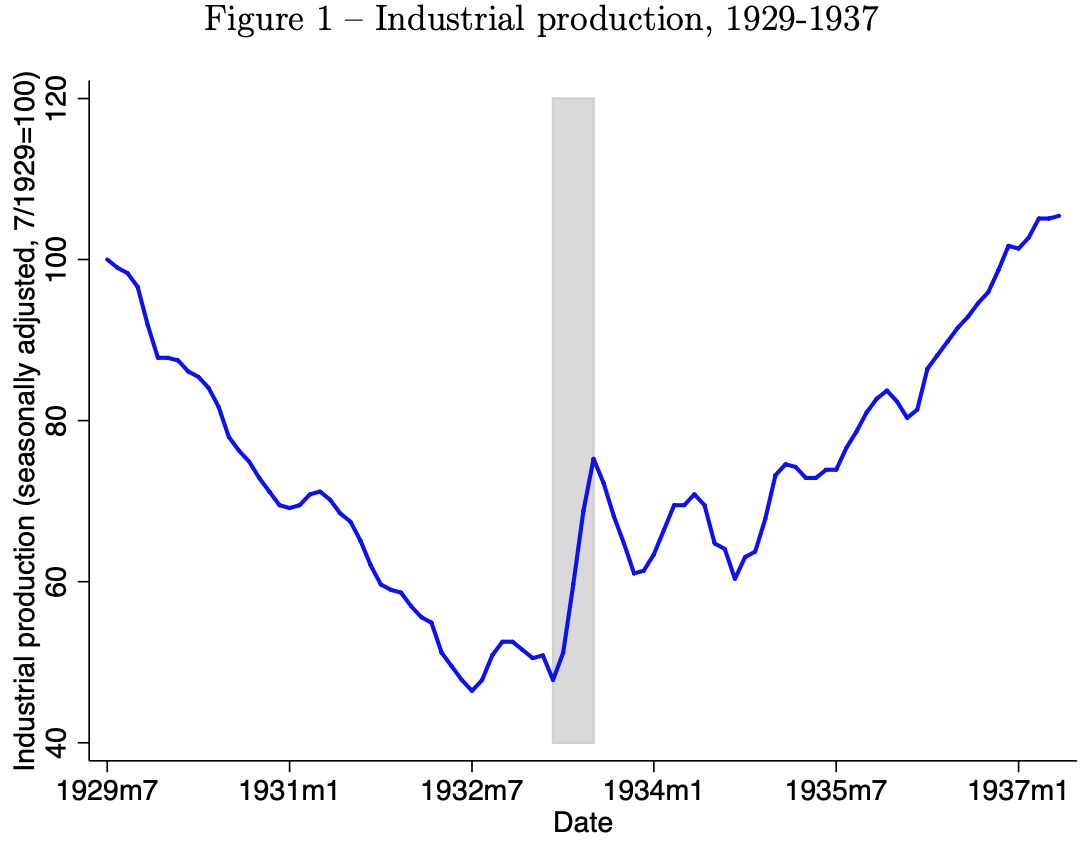
\includegraphics[scale=0.5]{figures/HRWFIG1.png}
\end{frame}

\begin{frame}
\frametitle[alignment=center]{Large Devaluation from Leaving Gold Standard}
\centering
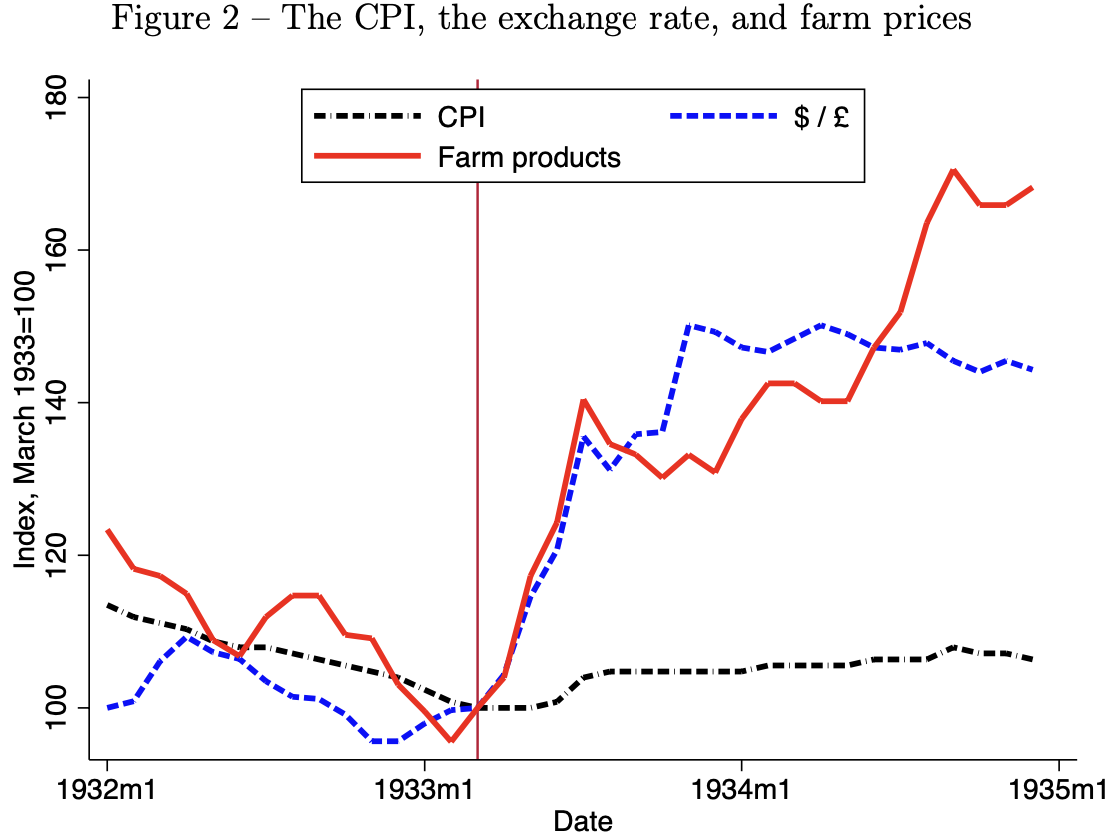
\includegraphics[scale=0.5]{figures/HRWFIG2.png}
\end{frame}

\begin{frame}
\frametitle[alignment=center]{Tradable Prices Rose}
\centering
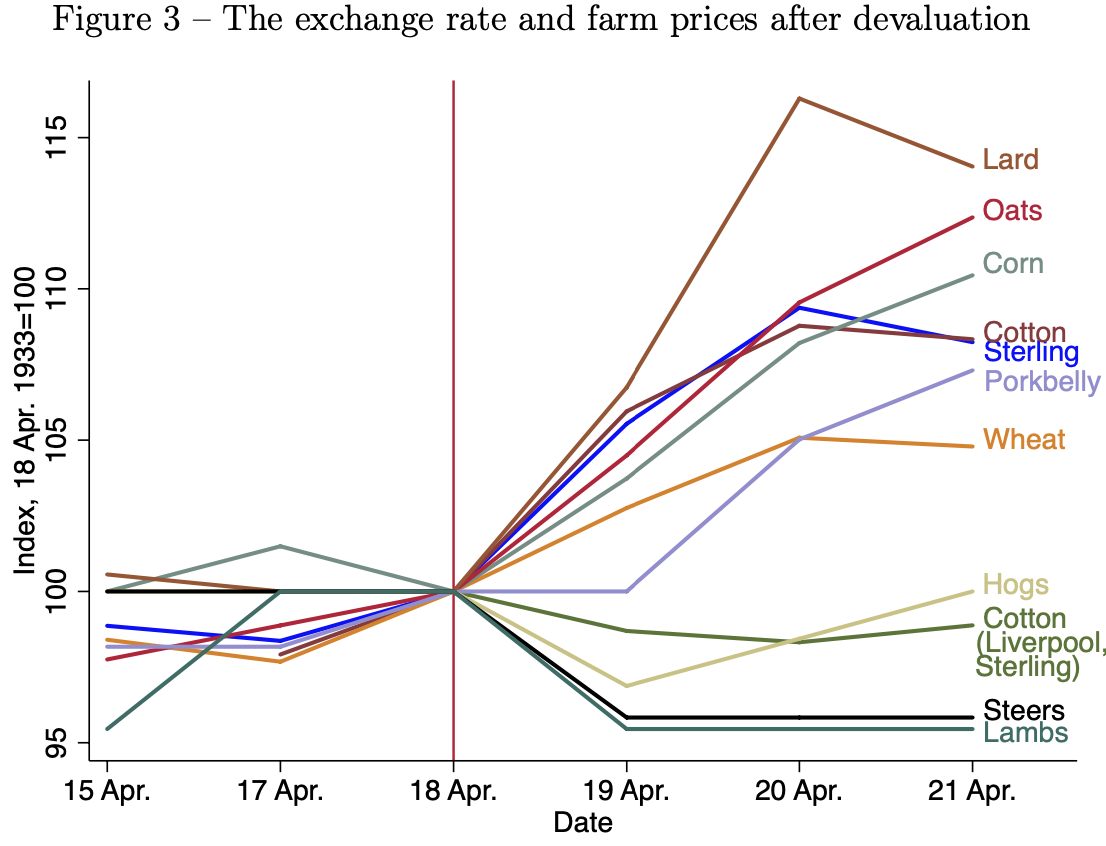
\includegraphics[scale=0.5]{figures/HRWFIG3.png}
\end{frame}

\begin{frame}
\frametitle[alignment=center]{Farm Incomes Rose}
\centering
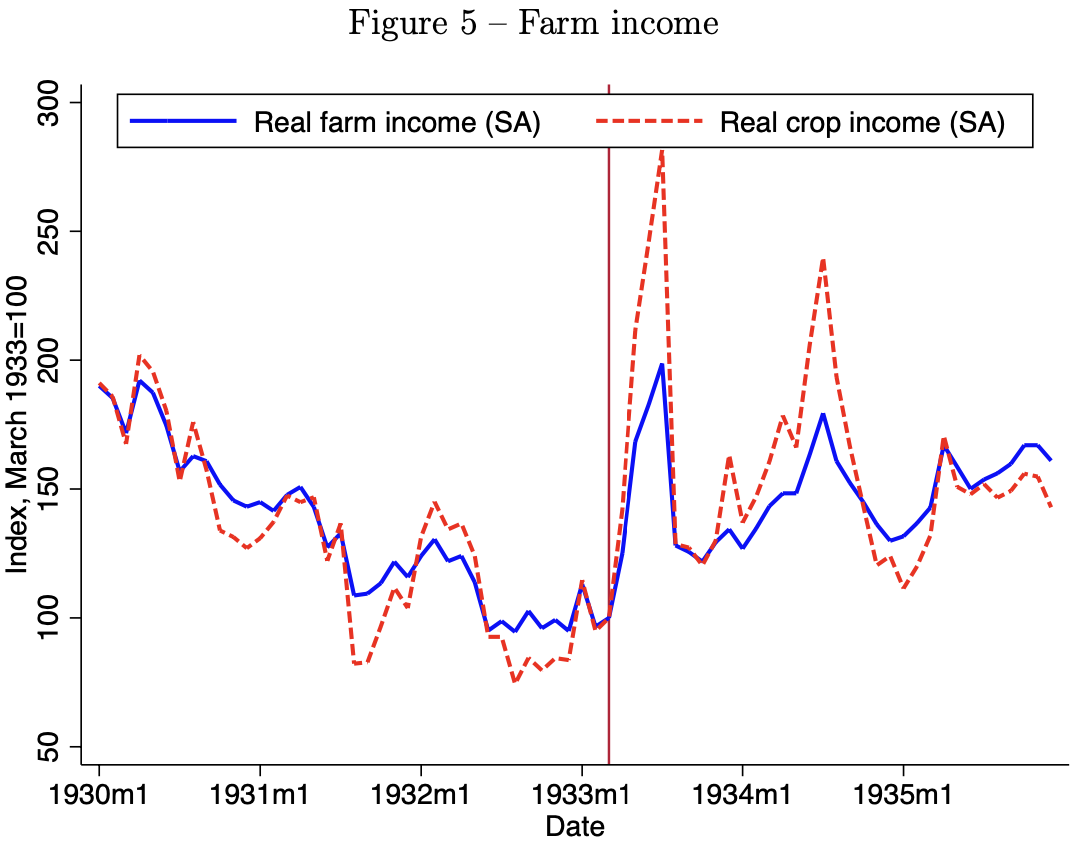
\includegraphics[scale=0.5]{figures/HRWFIG5.png}
\end{frame}


\begin{frame}
\frametitle[alignment=center]{Specification}
\begin{itemize}
	\item Cross-sectional regression of the form:
	\begin{align*}
		\%\Delta \text{Auto sales}_{i,\text{Spring 1933}} = \beta_0 + \beta_1 \text{Agricultural exposure}_i + \gamma'X_i+\epsilon_i
	\end{align*}
	\item What is the identifying assumption?
	\item Comments? Concerns?
\end{itemize}
\end{frame}

\begin{frame}
\frametitle[alignment=center]{Farm States Grow Faster}
\centering
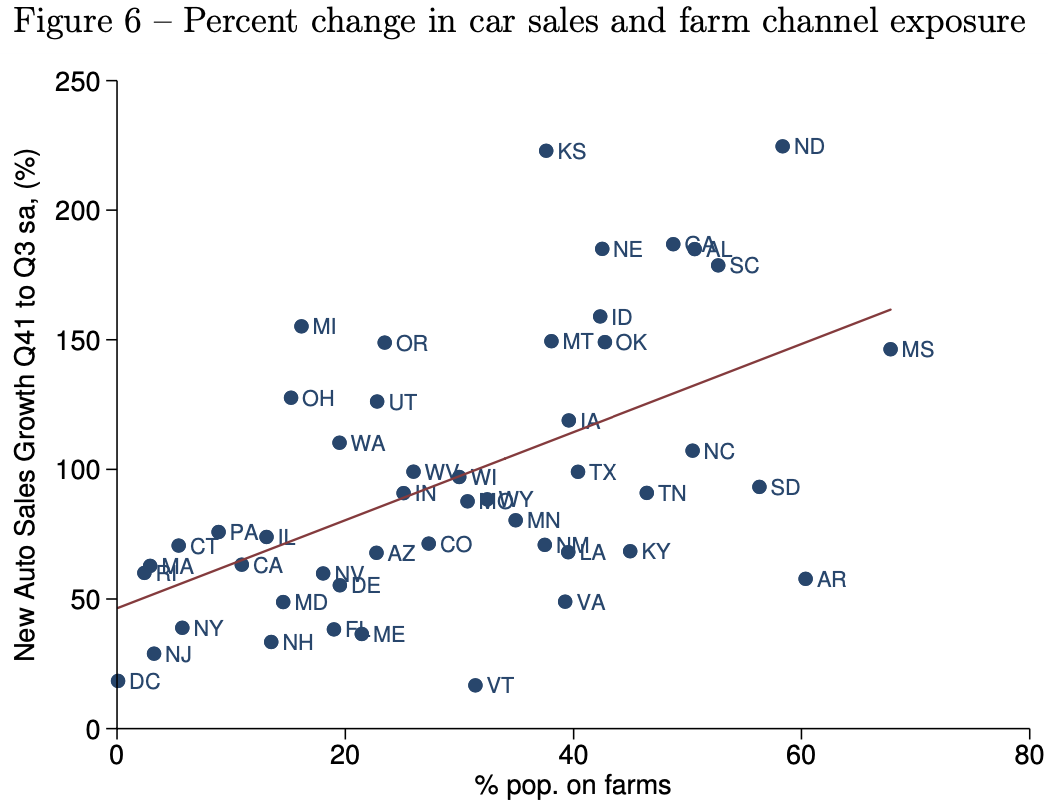
\includegraphics[scale=0.5]{figures/HRWFIG6a.png}
\end{frame}

\begin{frame}
\frametitle[alignment=center]{Test for Pre-Trends}
\centering
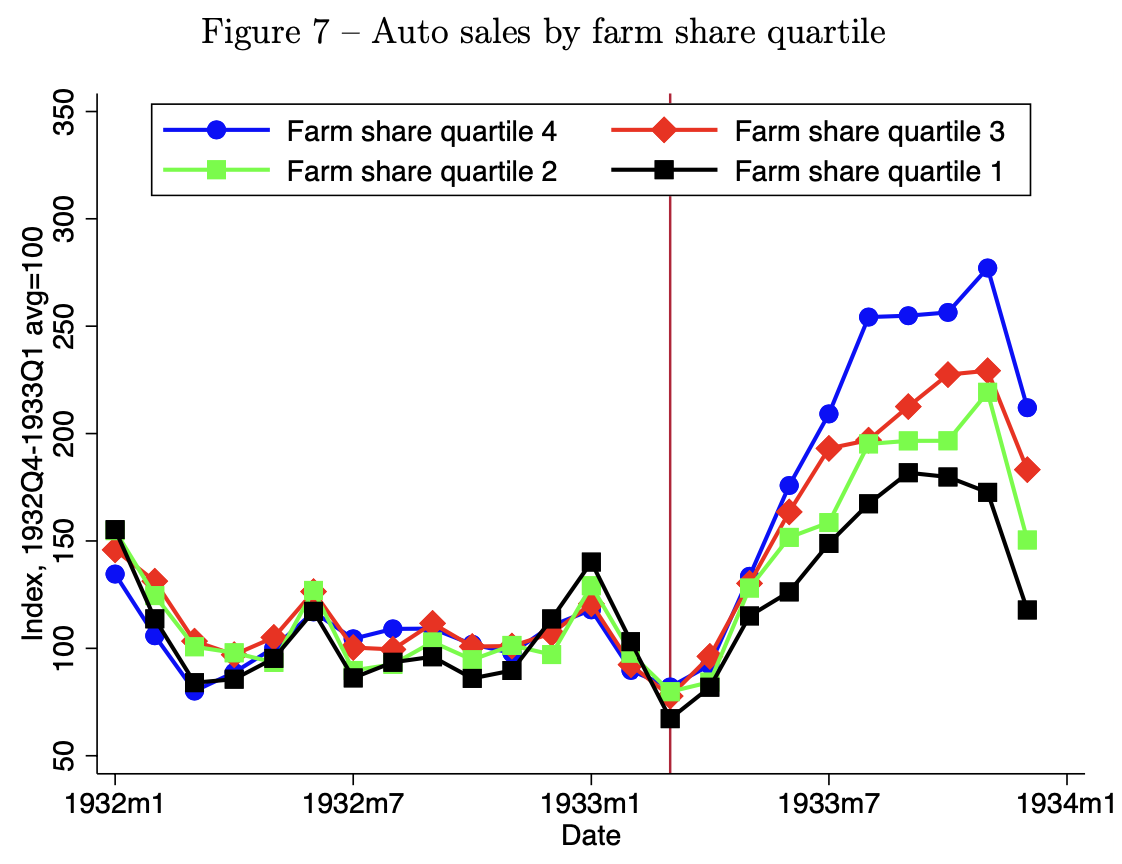
\includegraphics[scale=0.5]{figures/HRWFIG7.png}
\end{frame}

\begin{frame}
\frametitle[alignment=center]{County-level Analysis}
\centering
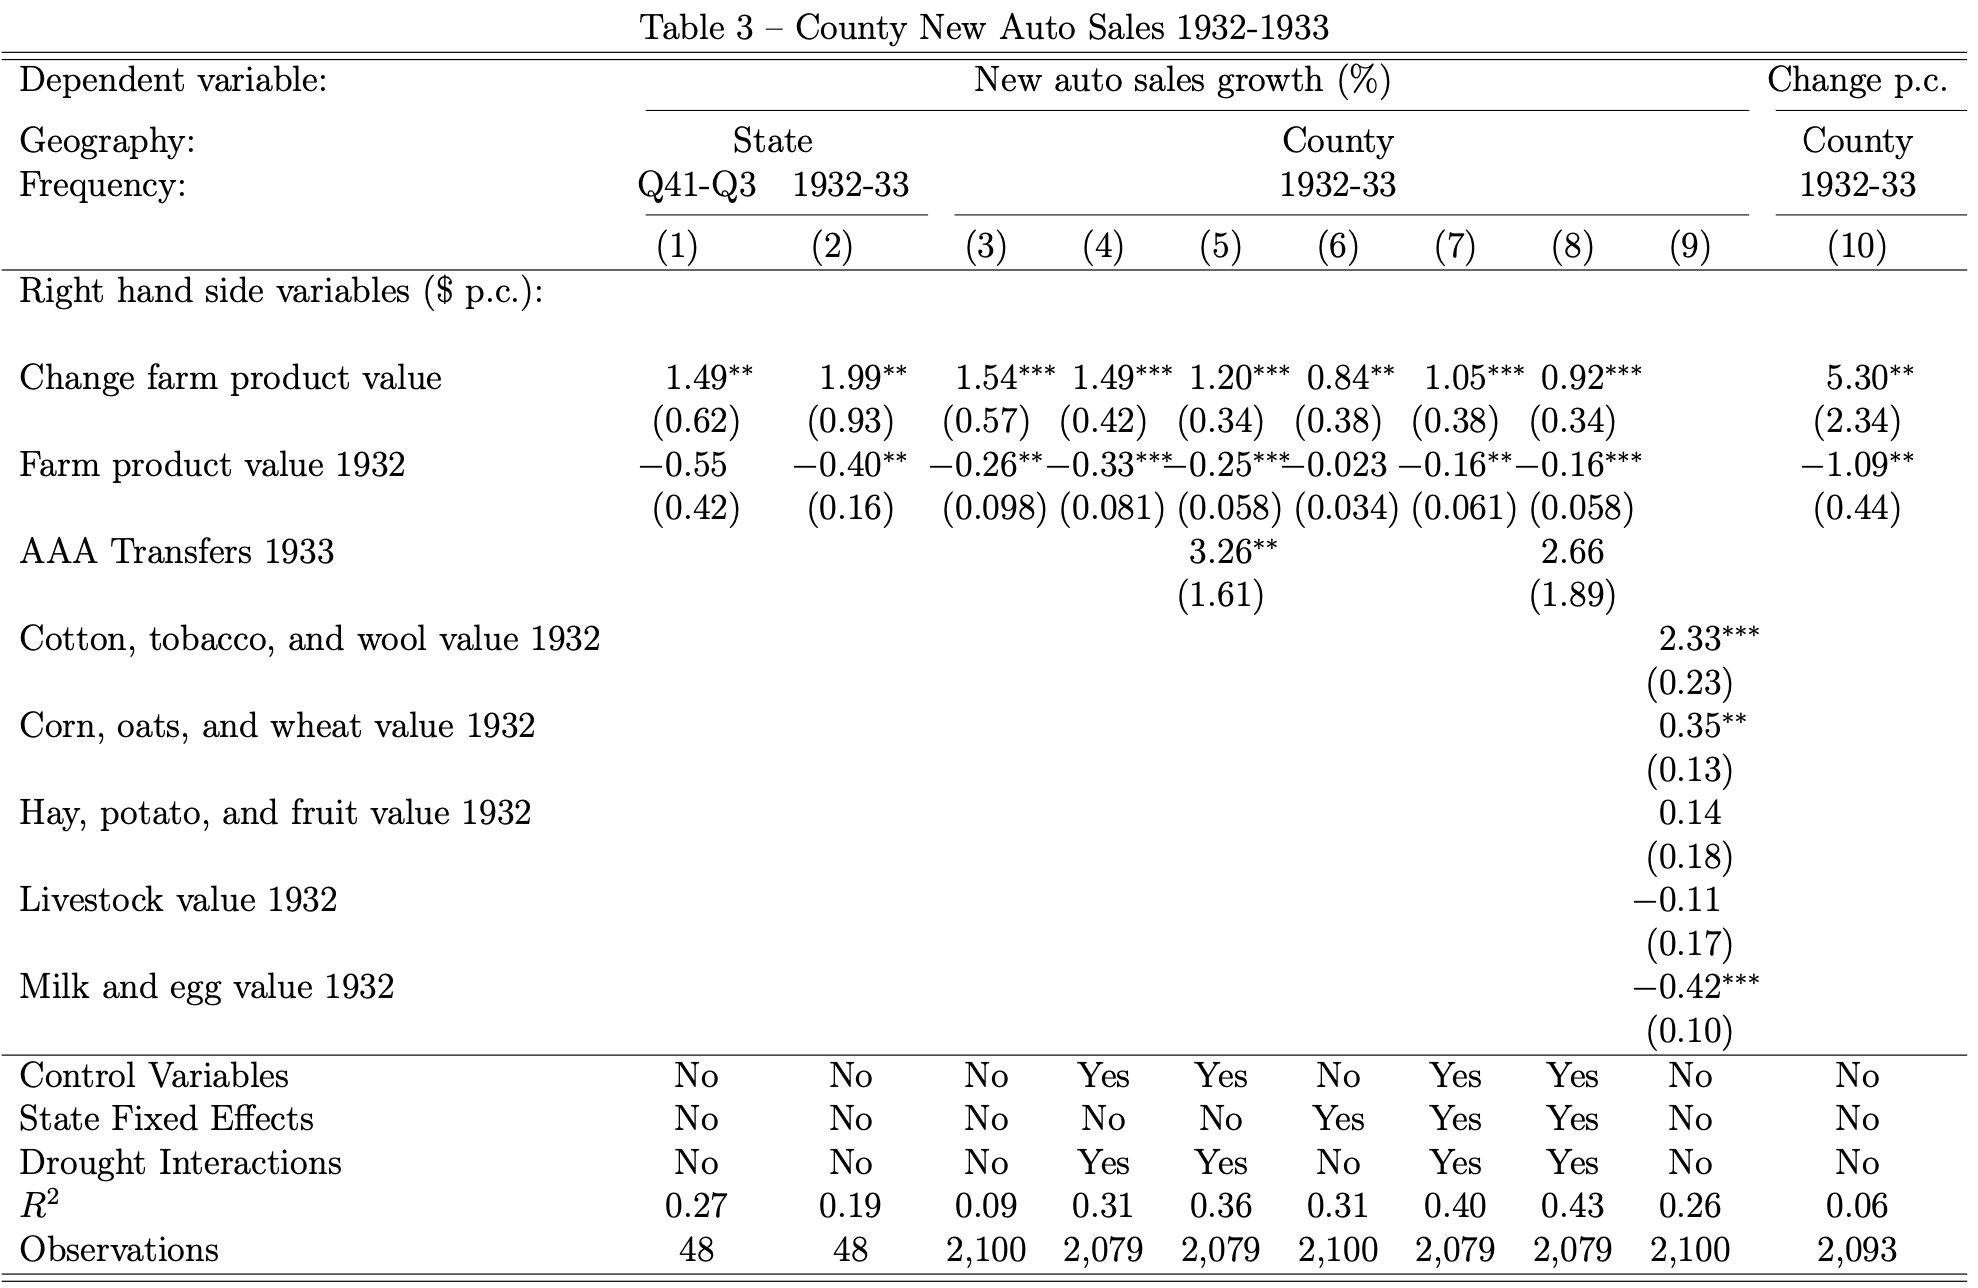
\includegraphics[scale=0.35]{figures/HRWTAB3.png}
\end{frame}

\begin{frame}
\frametitle[alignment=center]{Convincing?}

\end{frame}

\begin{frame}
\frametitle[alignment=center]{Aggregate Effects?}
\begin{itemize}
	\item Evidence is about \emph{relative} changes in consumption expenditure.
	\item Three mechanisms by which it can be expansionary overall:
	\begin{enumerate}
		\item Redistribution to higher-MPC households.
		\item Improves bank health.
		\item Raises inflation expectations.
	\end{enumerate}
\end{itemize}
\end{frame}

\begin{frame}
\frametitle[alignment=center]{Testing for Differential MPCs}
\begin{itemize}
	\item Cross-sectional regression of the form:
	\begin{align*}
		\%\Delta &\text{Auto sales}_{i,\text{Spring 1933}} =\\
		&  \beta_0 + \beta_1 \Delta\text{farm product value}_i \times \% \text{farms mortgaged} + \\ 
		&+ \beta_2 \text{farm product value}_i \times \% \text{farms mortgaged} \\
		&+ \beta_3 \Delta\text{farm product value}_i  +\beta_4 \% \text{farms mortgaged} \\
		& + \beta_5 \Delta\text{farm product value}_i  + \gamma'X_i+\epsilon_i
	\end{align*}
	\item What is the identifying assumption?
	\item Comments? Concerns?
\end{itemize}
\end{frame}

\begin{frame}
\frametitle[alignment=center]{Debt-Interaction Positiv}
\centering
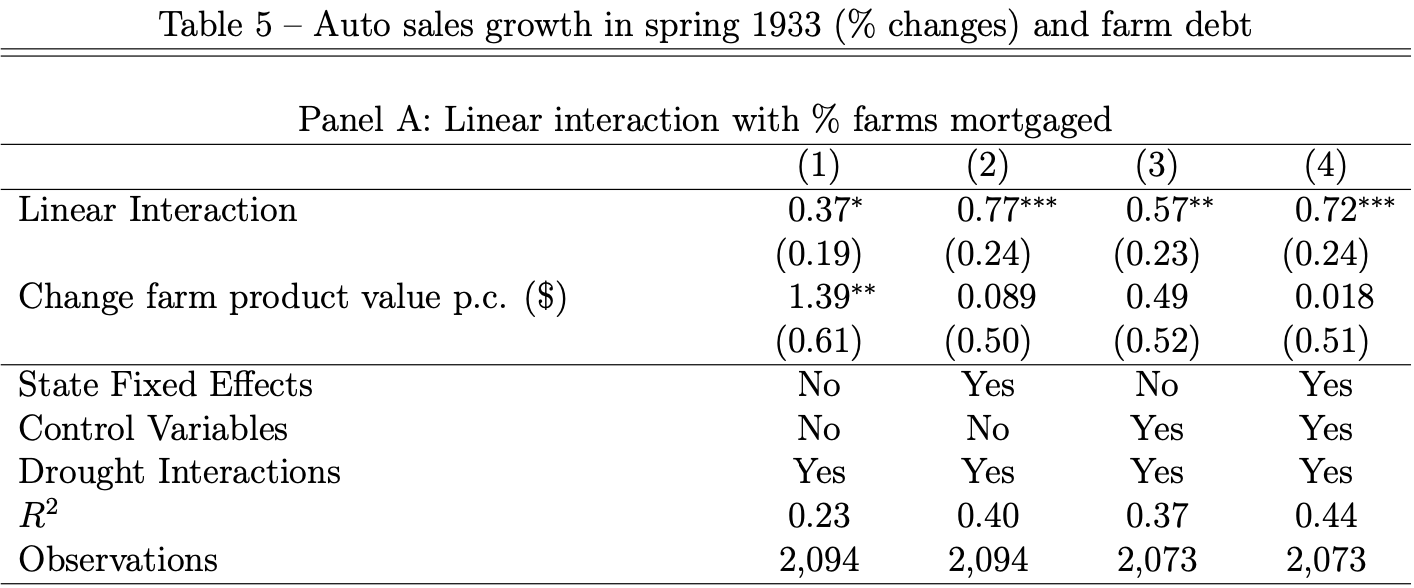
\includegraphics[scale=0.4]{figures/HRWTAB5a.png}
\end{frame}

\begin{frame}
\frametitle[alignment=center]{Differential Deposit Growth}
\centering
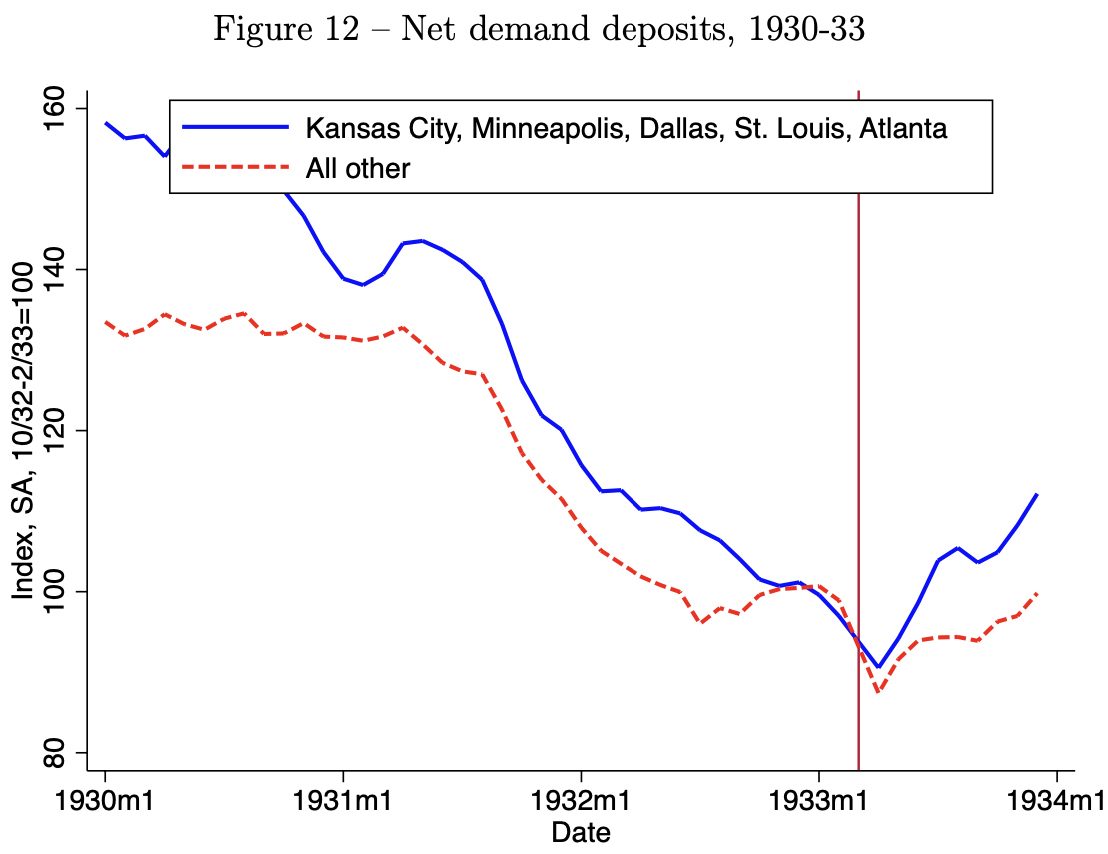
\includegraphics[scale=0.5]{figures/HRWFIG12.png}
\end{frame}

\begin{frame}
\frametitle[alignment=center]{Inflation Expectations?}
\centering
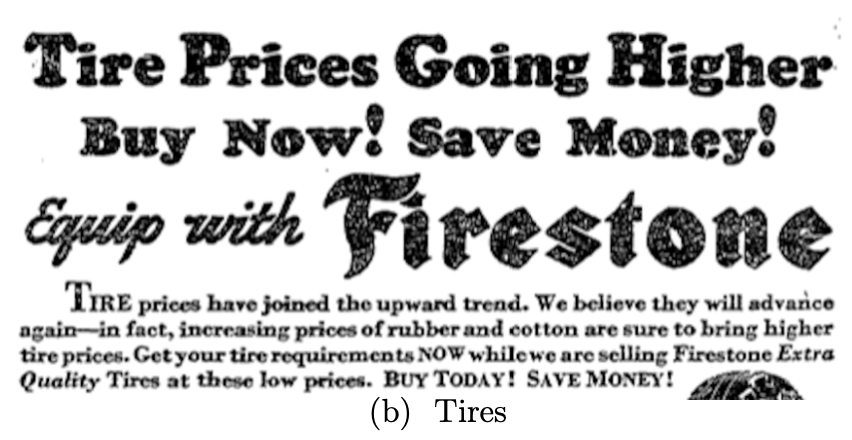
\includegraphics[scale=0.5]{figures/HRWFIG14b.png}
\end{frame}

\begin{frame}
\frametitle{Aggregation}

\begin{itemize}
\item Simple framework to examine how cross-sectional estimates map to the aggregate economy.
\item Model has heterogeneity on the following three dimensions:
\begin{itemize}
	\item Income from farming, labor, or pricing power.
	\item Permanent income vs hand-to-mouth.
	\item Farm vs urban area.
\end{itemize}
\item Simplifications:
\begin{itemize}
	\item Model essentially static.
	\item Exogenous relative price movements.
\end{itemize}
\item Who looked at the appendix?
\end{itemize}

\end{frame}

\begin{frame}
\frametitle{Key result}
\vspace{-0.8cm}
\begin{align*}
	\% \Delta \text{Cars} &= \underbrace{\beta \times
                         \phi^{f}}_{\substack{\text{``naive''} \\
  \text{extrapolation}}} \times  \underbrace{\frac{\text{Farm
  area income per capita}}{\text{National income per
  capita}}}_{\text{Relative income p.c.}} \\
  & \times  \underbrace{\left( 1-\xi\frac{\theta^{w}}{\theta^{f}} \right)}_{\substack{\text{Redistribution from } \\ \text{high-MPC consumers}}} \times \underbrace{\mu_{t}}_{\substack{\text{Aggregate}\\ \text{spending}\\ \text{multiplier}}} \\
  &\qquad  + \underbrace{-\sigma  d\ln (1+r_t)}_{\text{Intertemporal Substitution}}
\end{align*}
\begin{itemize}
	\item Comments? Concerns?
\end{itemize}

\end{frame}

\begin{frame}
\frametitle[alignment=center]{Aggregate Effect of Farm Channel}
\centering
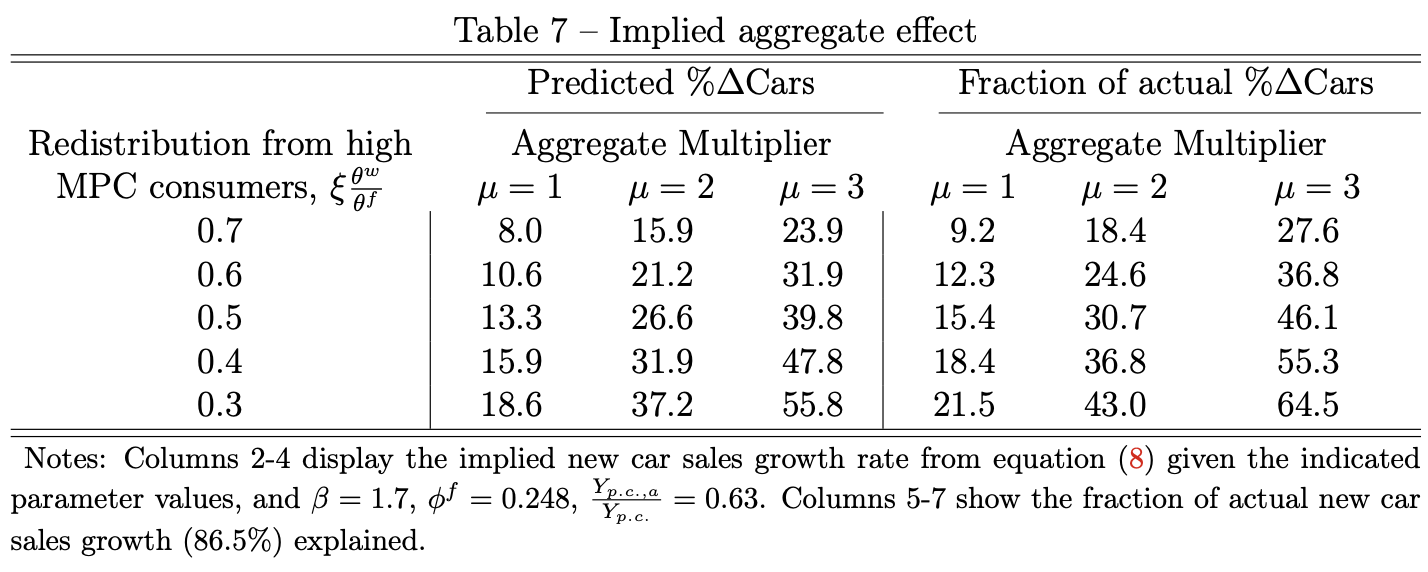
\includegraphics[scale=0.4]{figures/HRWTAB7.png}
\begin{itemize}
	\item Thoughts? Comments?
\end{itemize}
\end{frame}

\begin{frame}
\frametitle[alignment=center]{Convincing?}

\end{frame}

% %%%%%%%%%%%%%%%%%%%%%%%%%%%%%%%%%%%%%%%%%%%%%%%%%%
% \section{Cloyne, Ferreira, and Surico (2020, ReStud)}
% %%%%%%%%%%%%%%%%%%%%%%%%%%%%%%%%%%%%%%%%%%%%%%%%%%

% \begin{frame}
% \frametitle[alignment=center]{Data}
% \begin{itemize}
% 	\item Monetary shocks for U.S., U.K.
% 	\item Consumer expenditure data.
% 	\begin{itemize}
% 		\item Detailed data on consumption.
% 		\item More rudimentary data on income and especially wealth.
% 		\item Contains information on housing tenure and housing debt status.
% 	\end{itemize}
% \end{itemize}
% \end{frame}


% \begin{frame}
% \frametitle[alignment=center]{Aggregate Monetary Shock}
% \centering
% 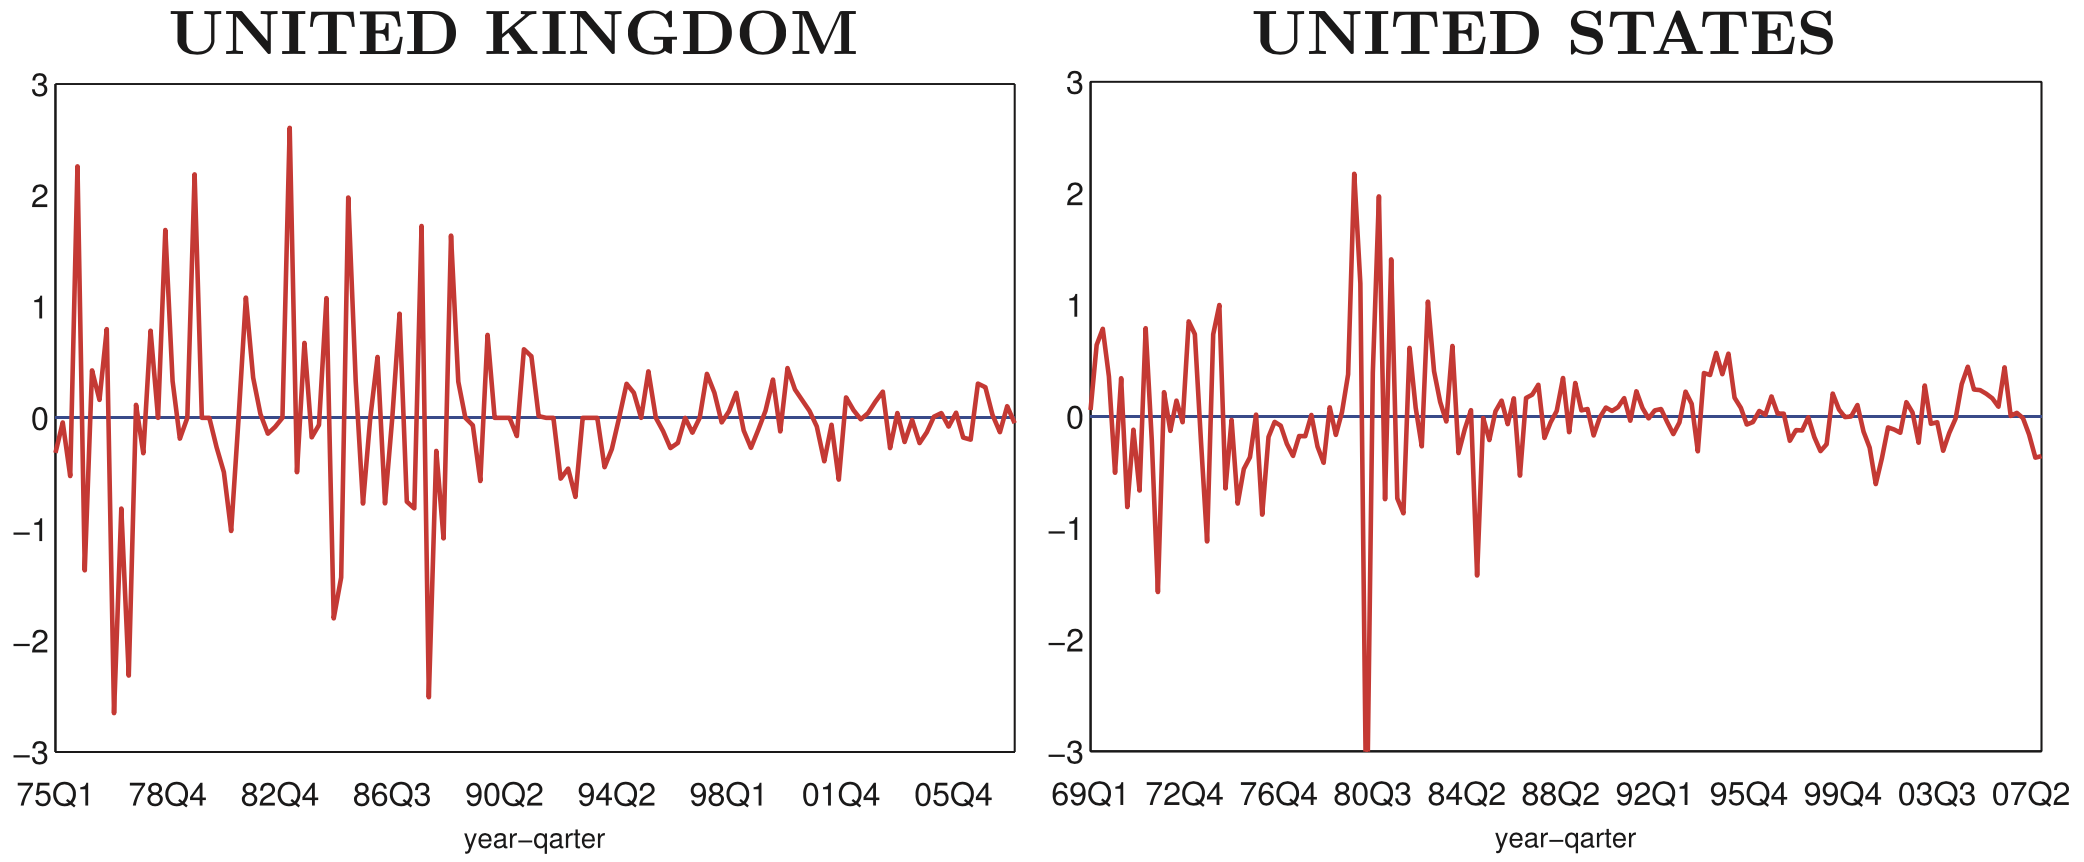
\includegraphics[scale=0.3]{figures/CFSFIG2.png}
% \begin{itemize}
% 	\item Thoughts? Comments?
% \end{itemize}
% \end{frame}

% \begin{frame}
% \frametitle[alignment=center]{Specification}
% \begin{align*}
% 	X_{i,t} = \alpha_0^i + \alpha_1^i trend + B^i(L)X_{i,t-1} + C^i(L)S_{t-1} + \sum_{q=2}^{4}D_q^i Z_q + u_{i,t}
% \end{align*}
% \begin{itemize}
% 	\item $i \in$ [Mortgagor, Outright-Owner, Renter]
% 	\item Identification assumption?
% 	\item Comments? Concerns?
% \end{itemize}
% \end{frame}

% \begin{frame}
% \frametitle[alignment=center]{Nondurable Expenditure}
% \centering
% 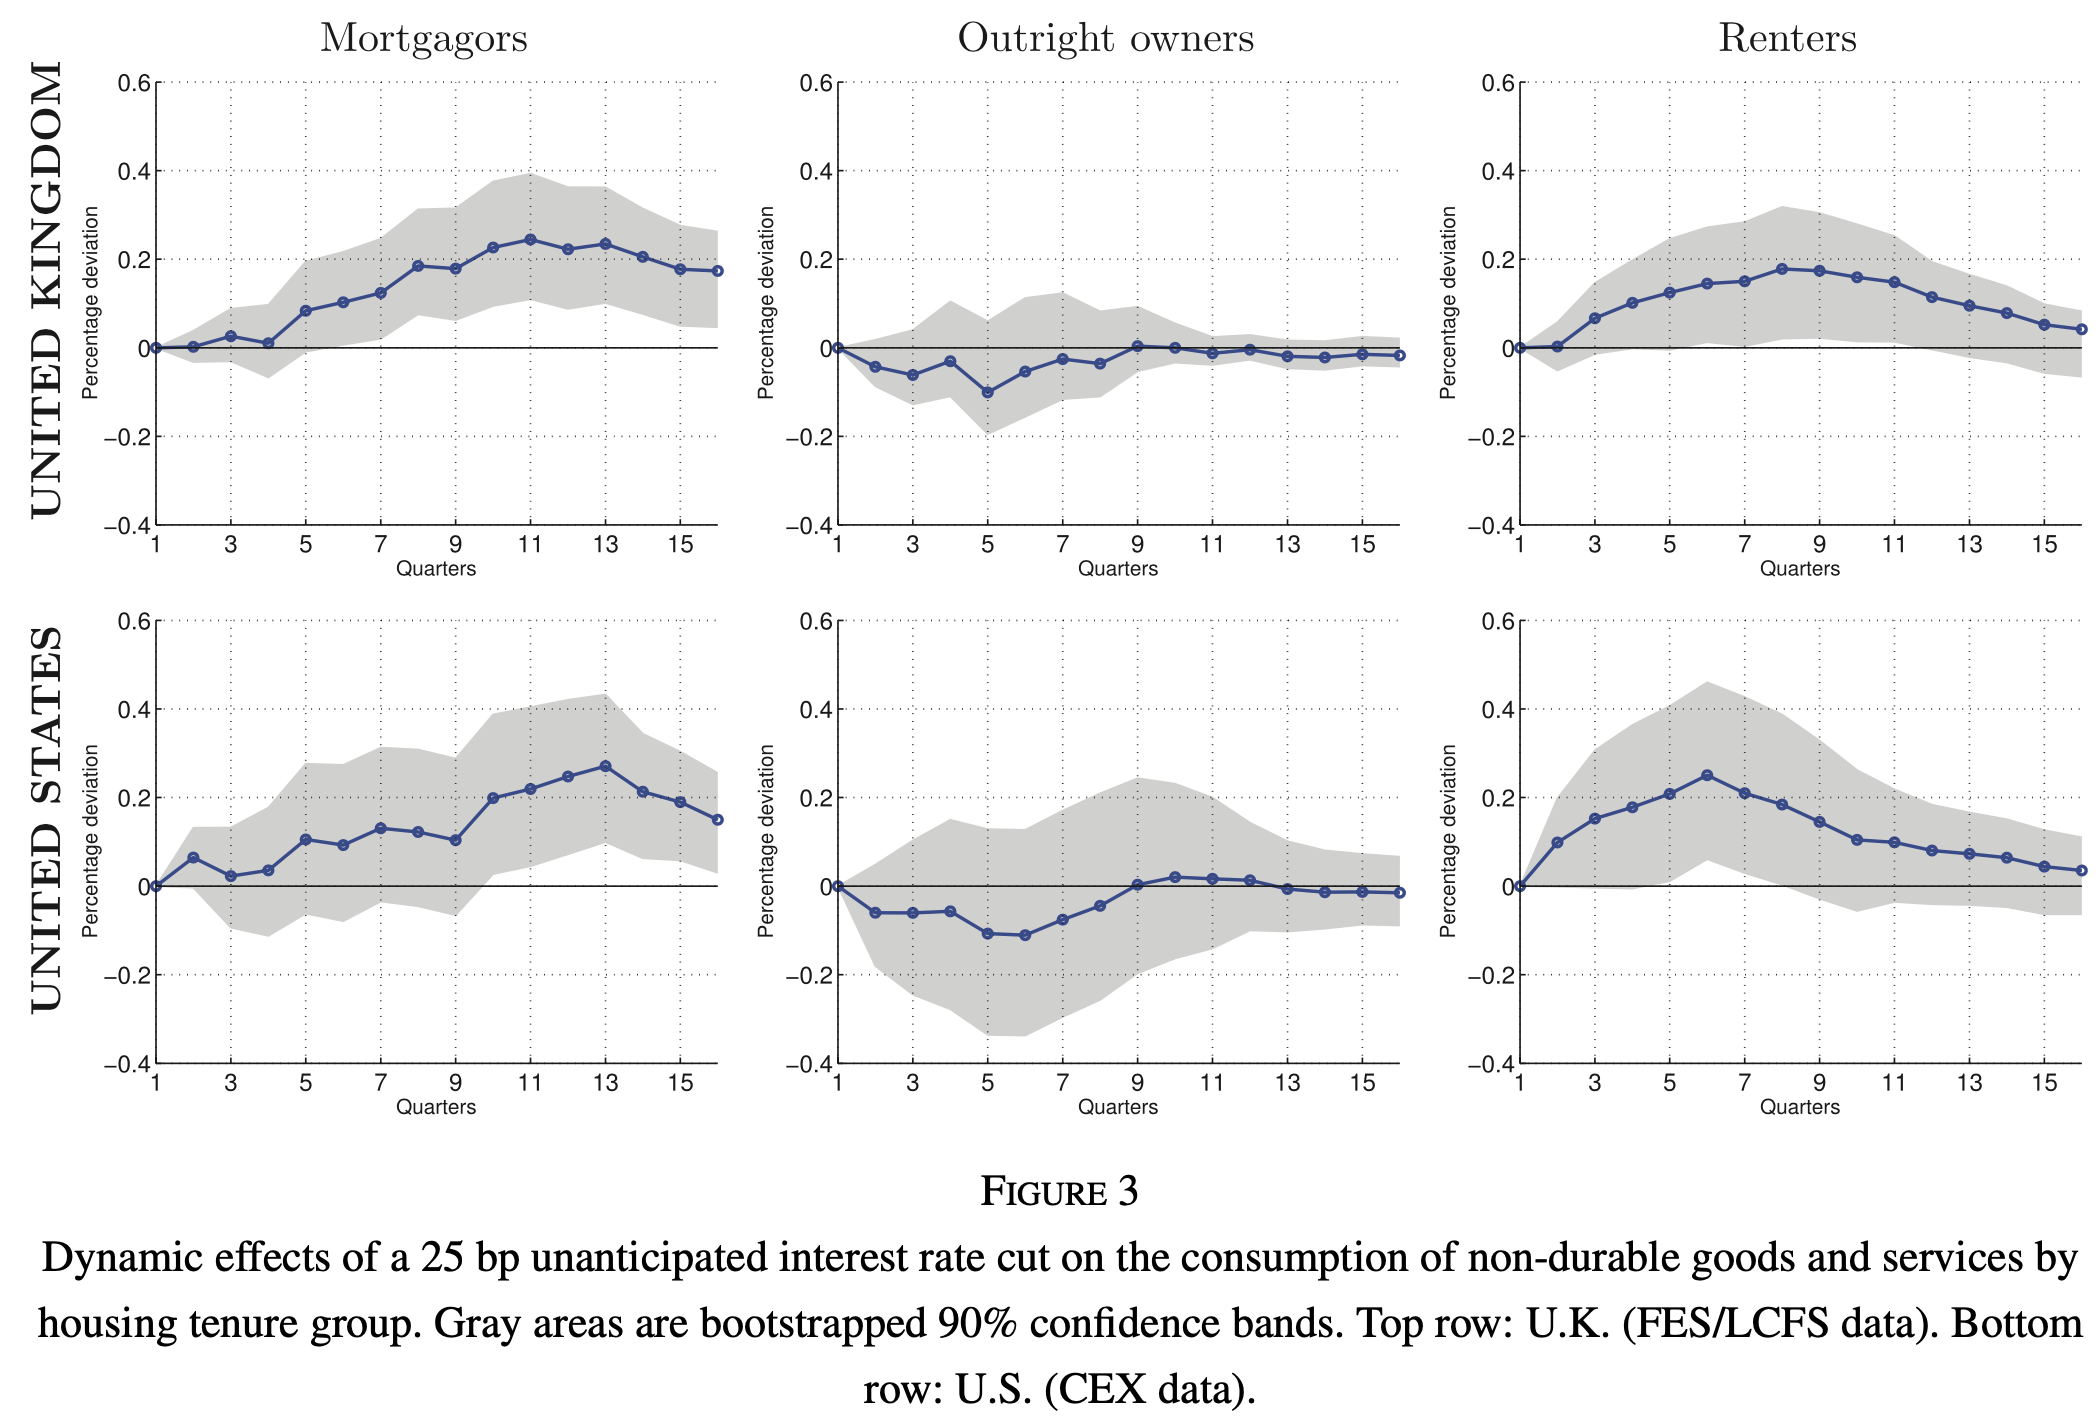
\includegraphics[scale=0.3]{figures/CFSFIG3.png}
% \end{frame}

% \begin{frame}
% \frametitle[alignment=center]{Durable Expenditure}
% \centering
% 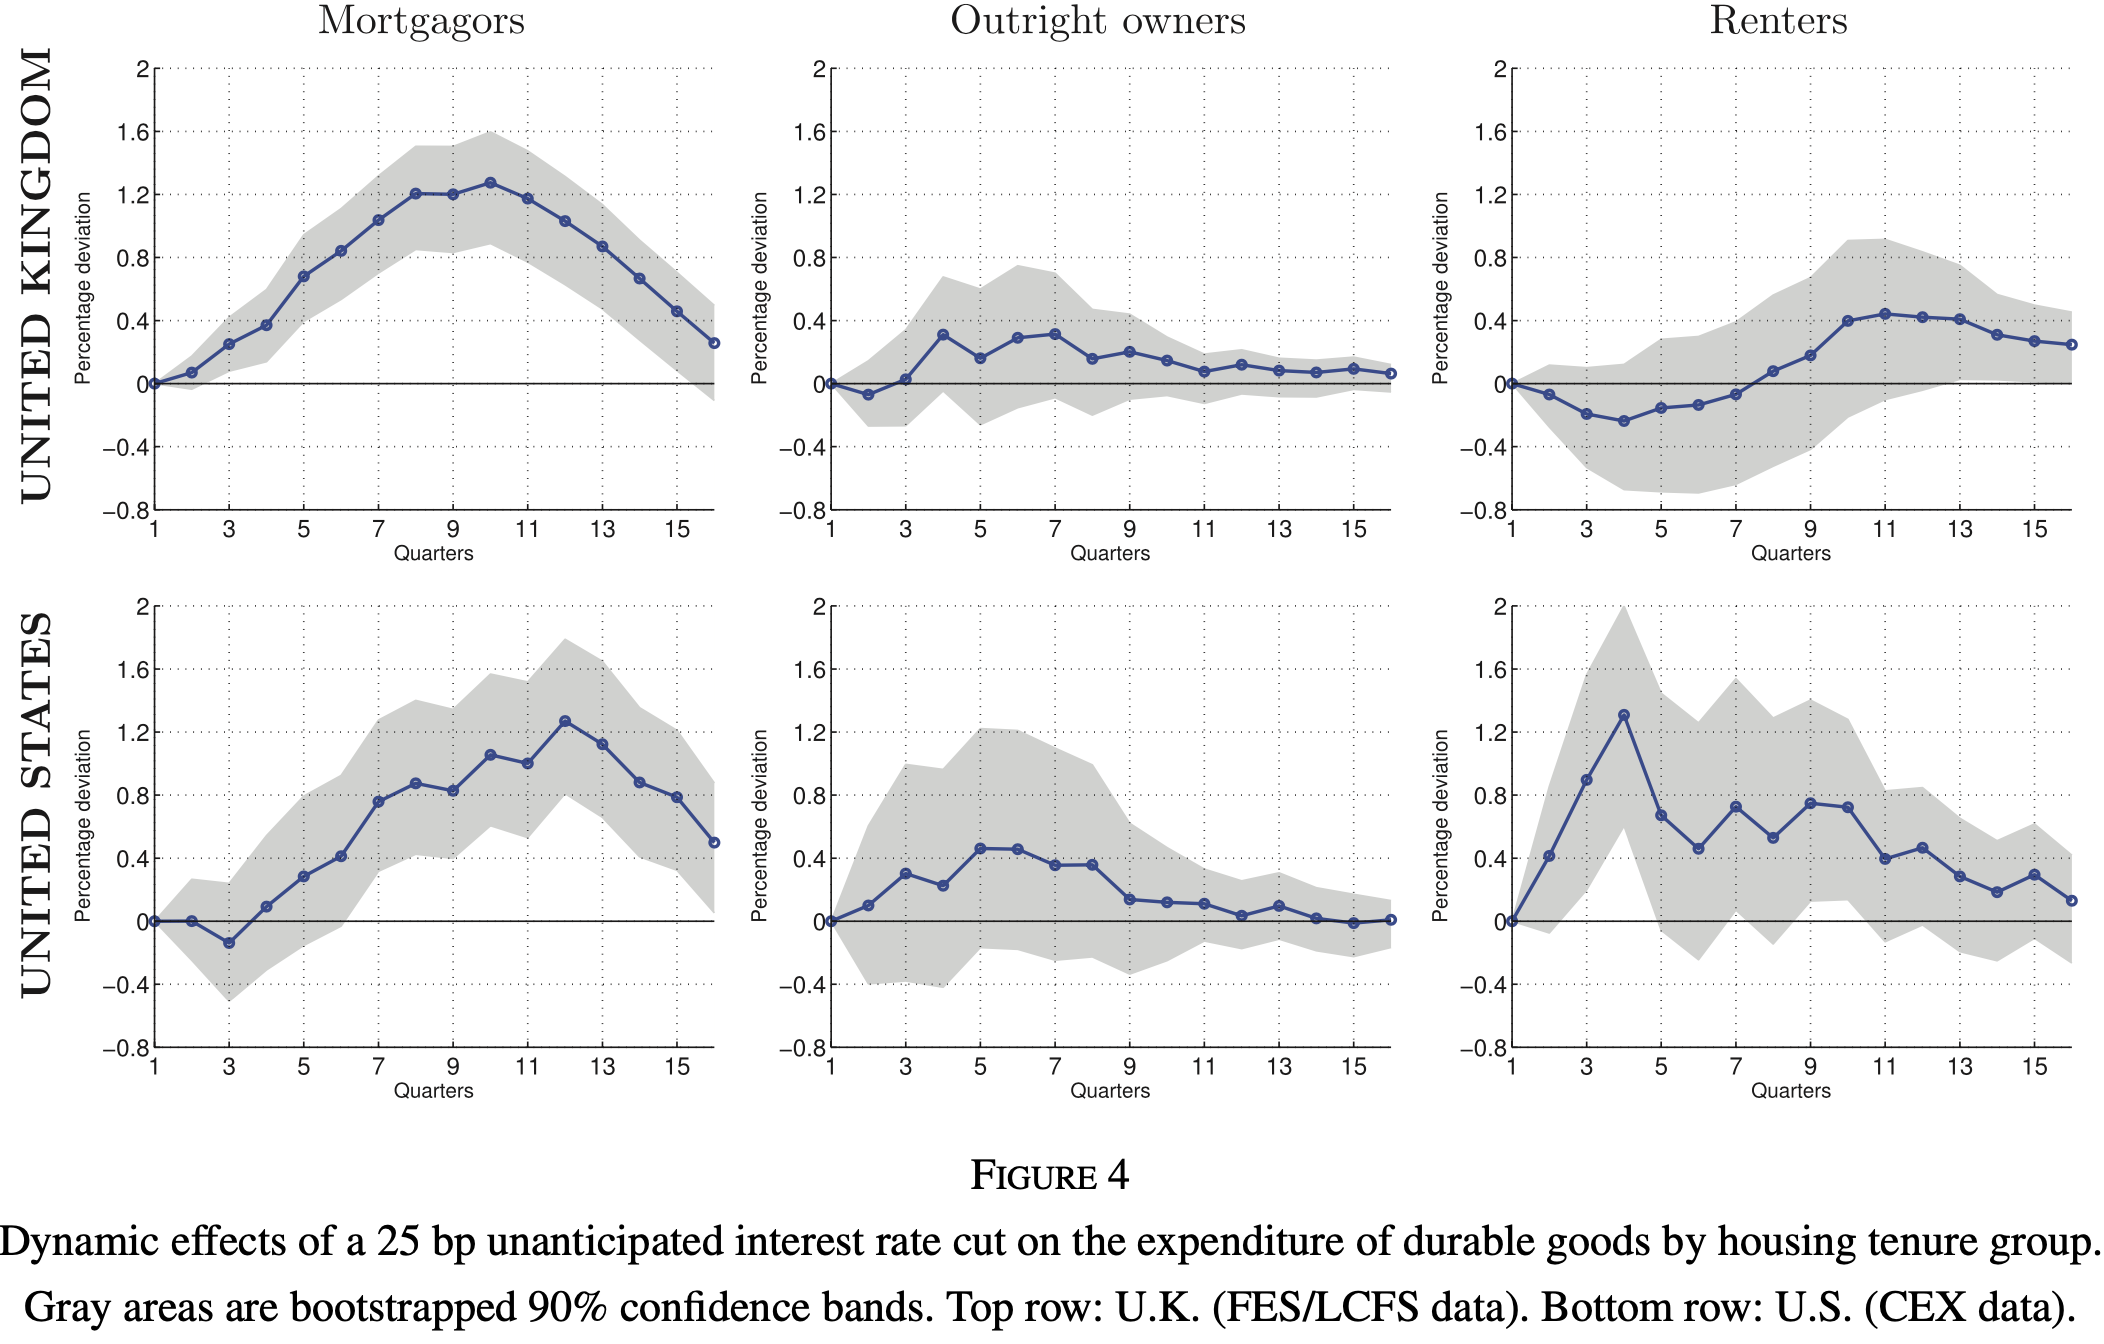
\includegraphics[scale=0.3]{figures/CFSFIG4.png}
% \end{frame}

% \begin{frame}
% \frametitle[alignment=center]{Comparison to Income}
% \centering
% 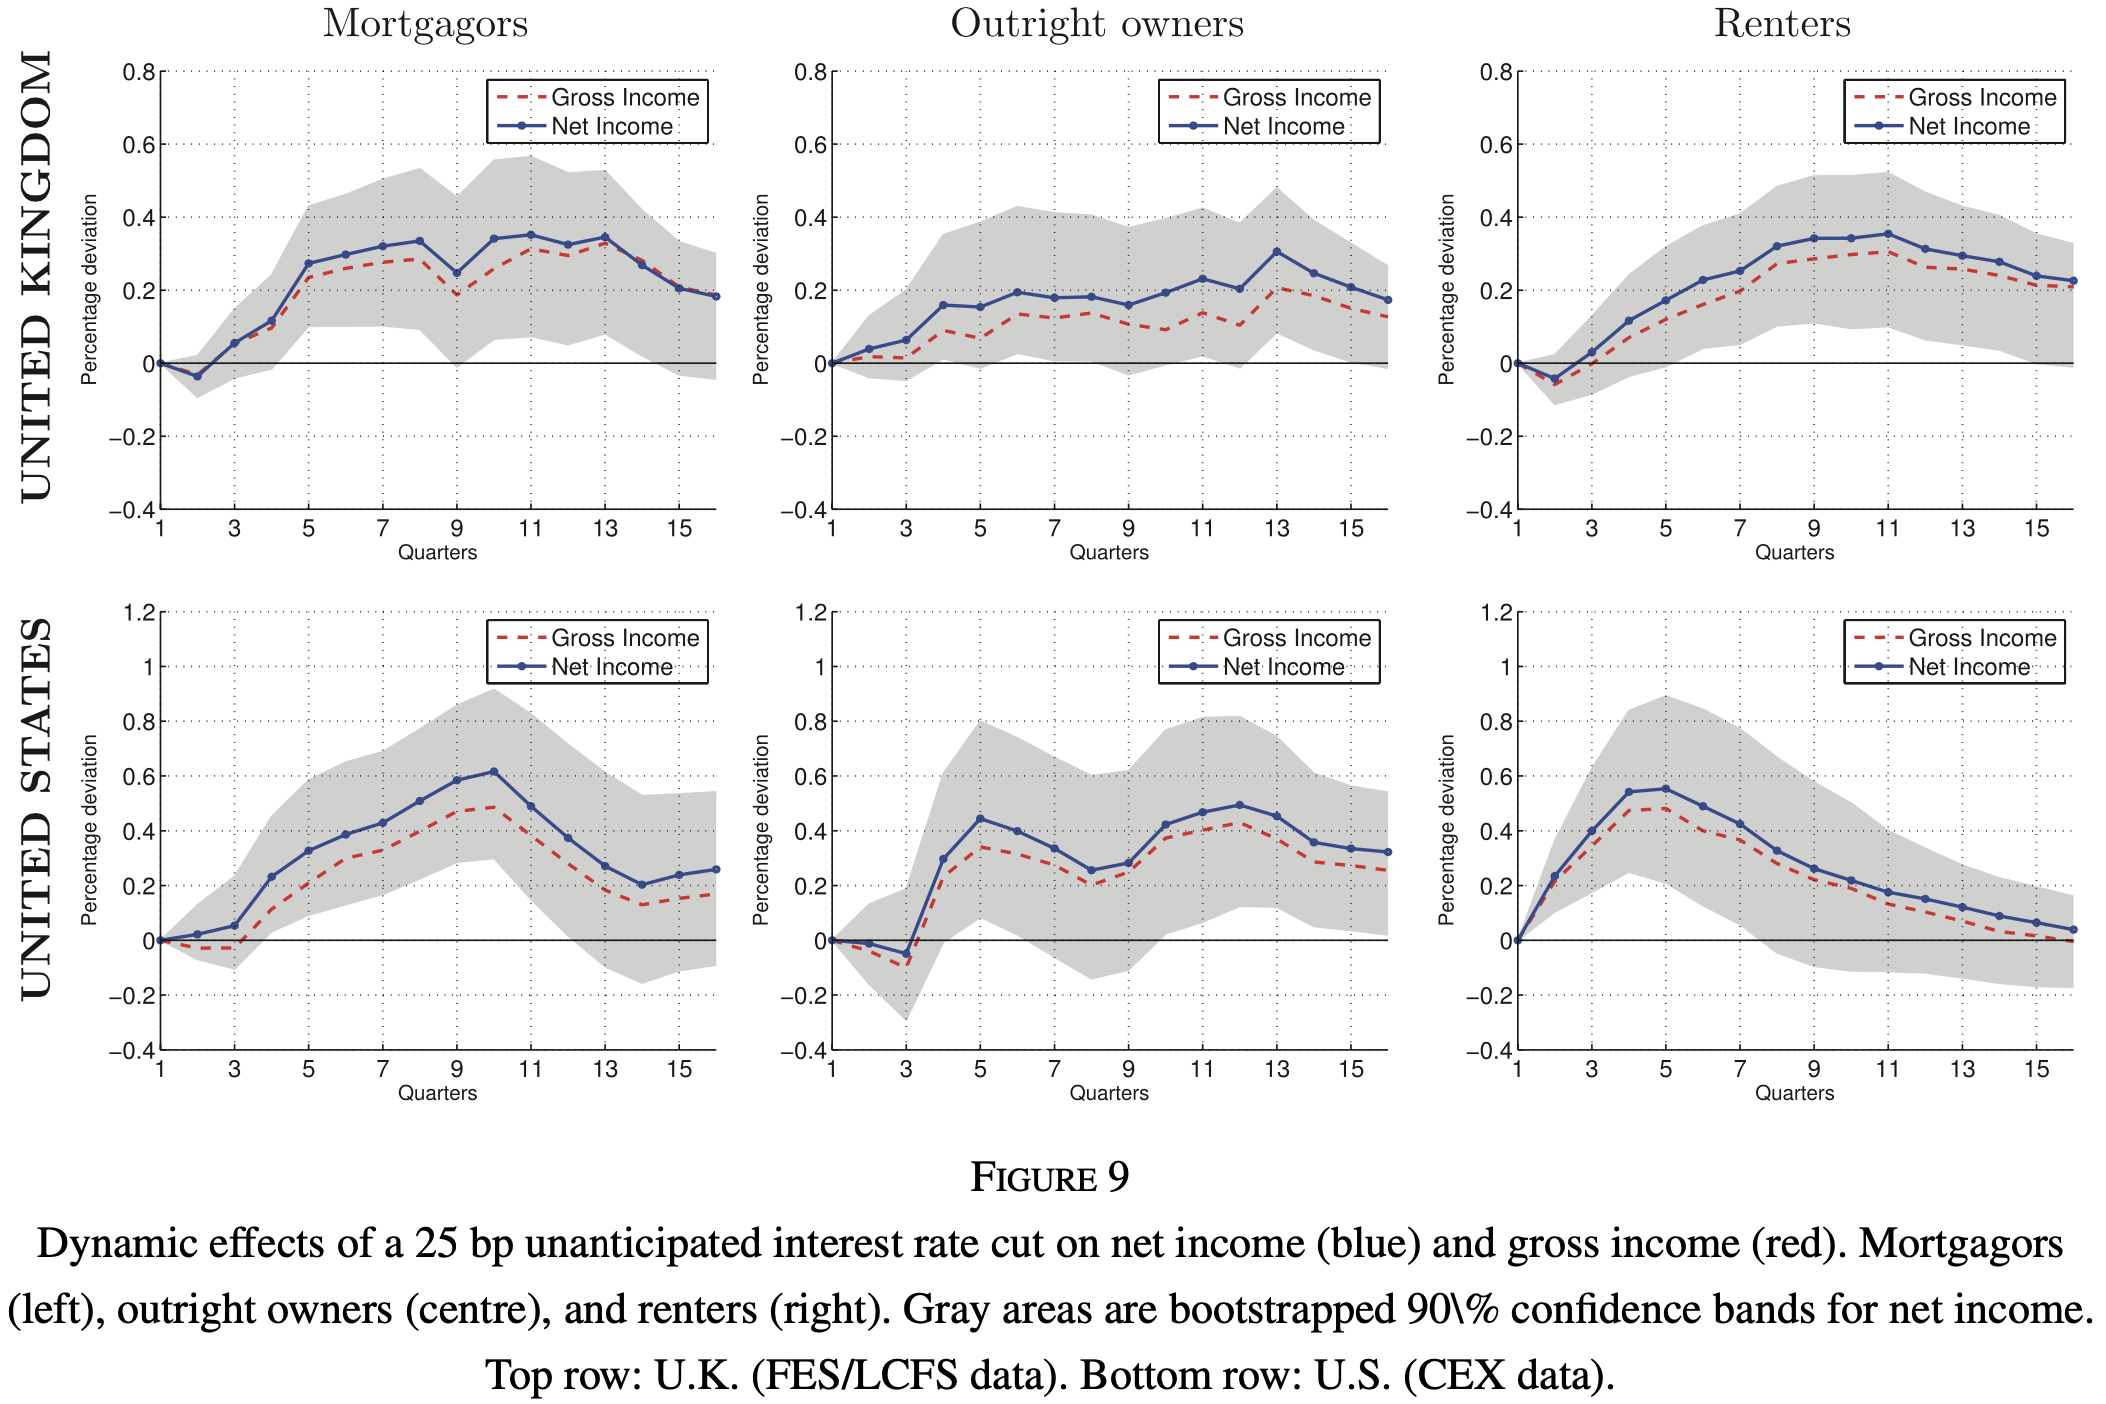
\includegraphics[scale=0.3]{figures/CFSFIG9.png}
% \end{frame}

% \begin{frame}
% \frametitle[alignment=center]{Comparison to Income}
% \centering
% 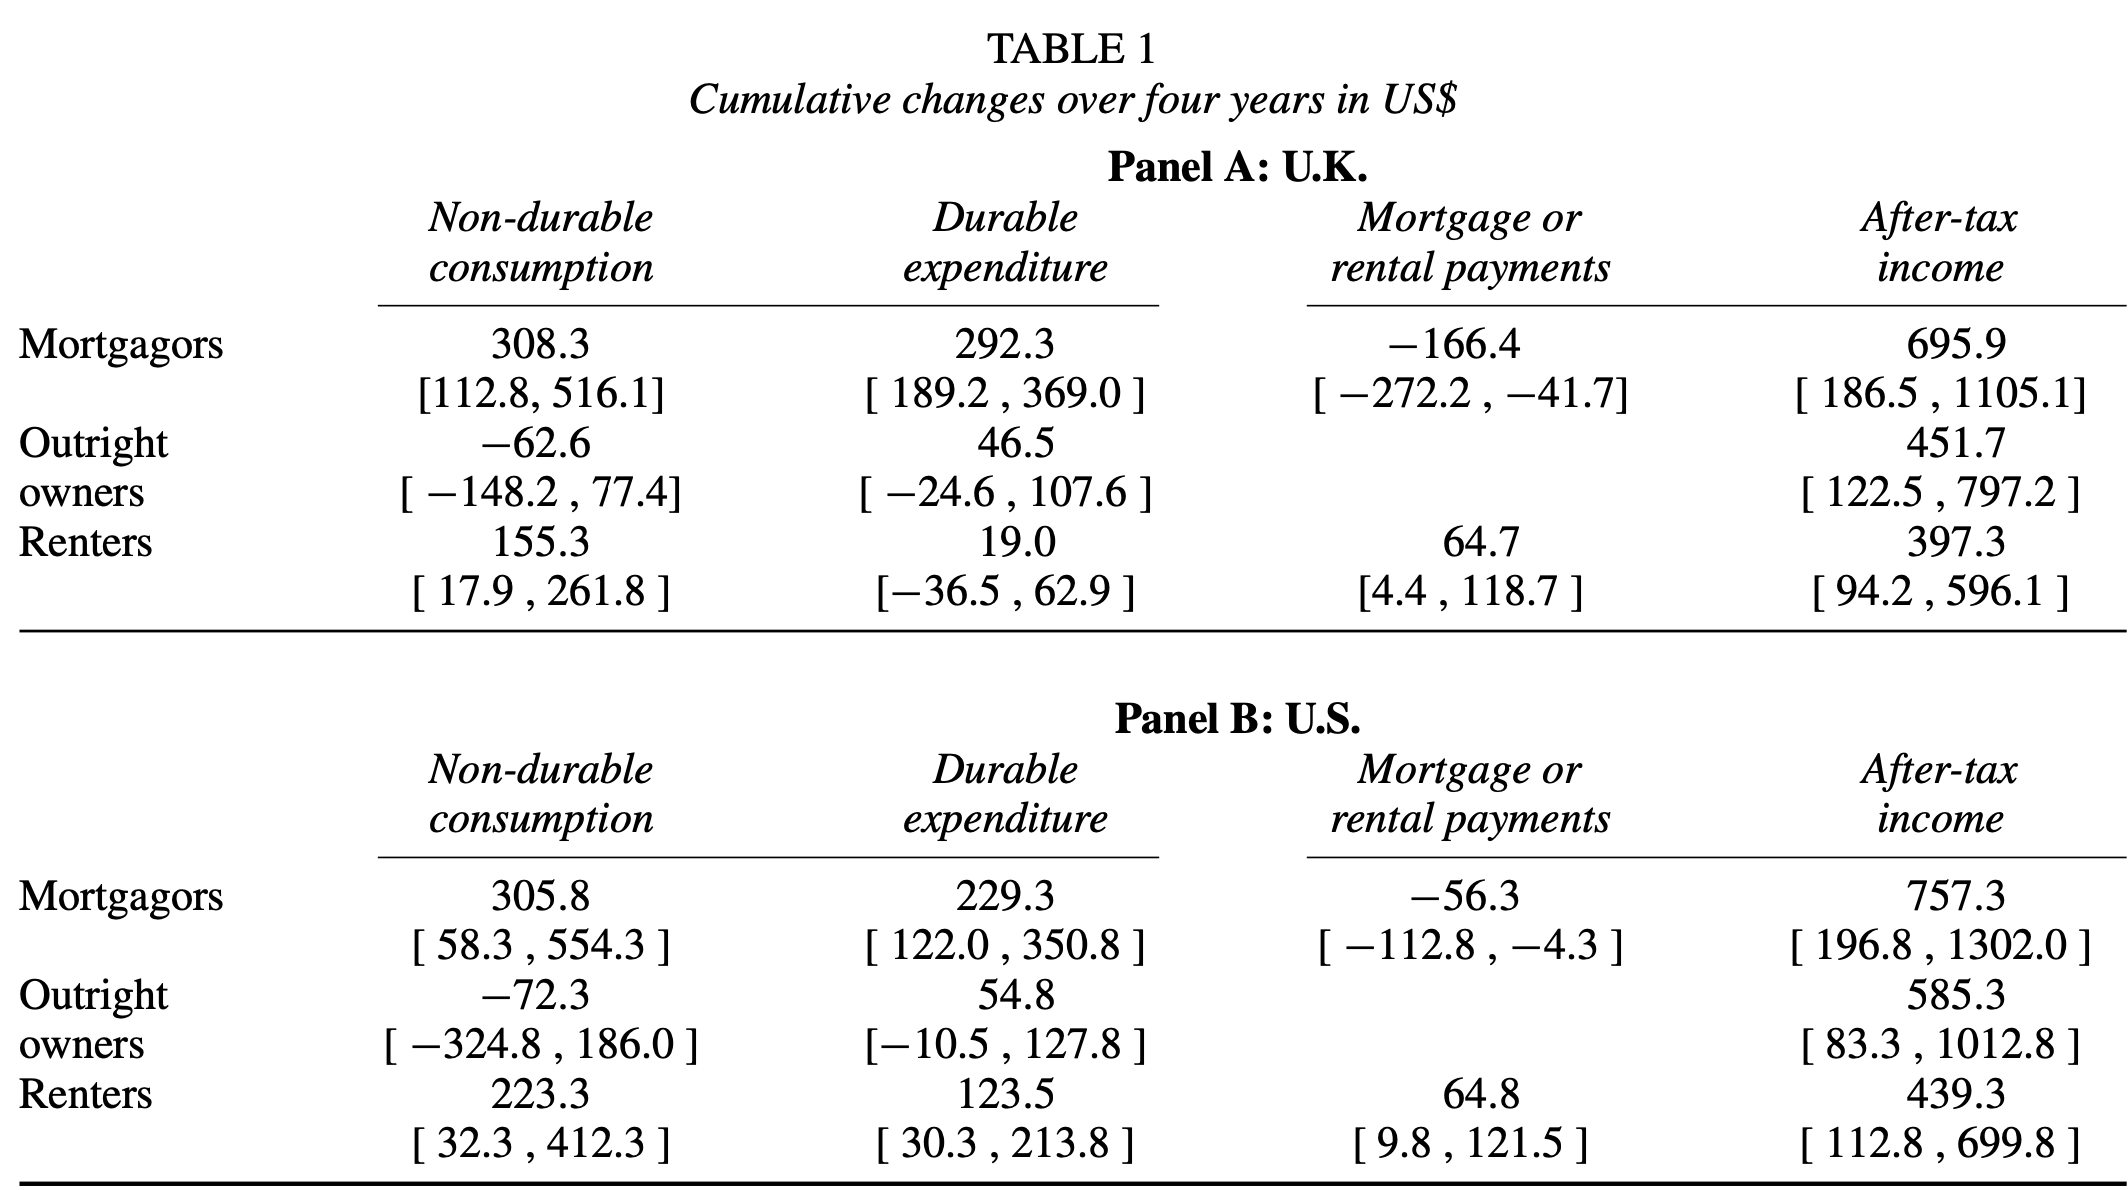
\includegraphics[scale=0.3]{figures/CFSTAB1.png}
% \end{frame}

% \begin{frame}
% \frametitle[alignment=center]{Demographic Sub-groups}
% \centering
% 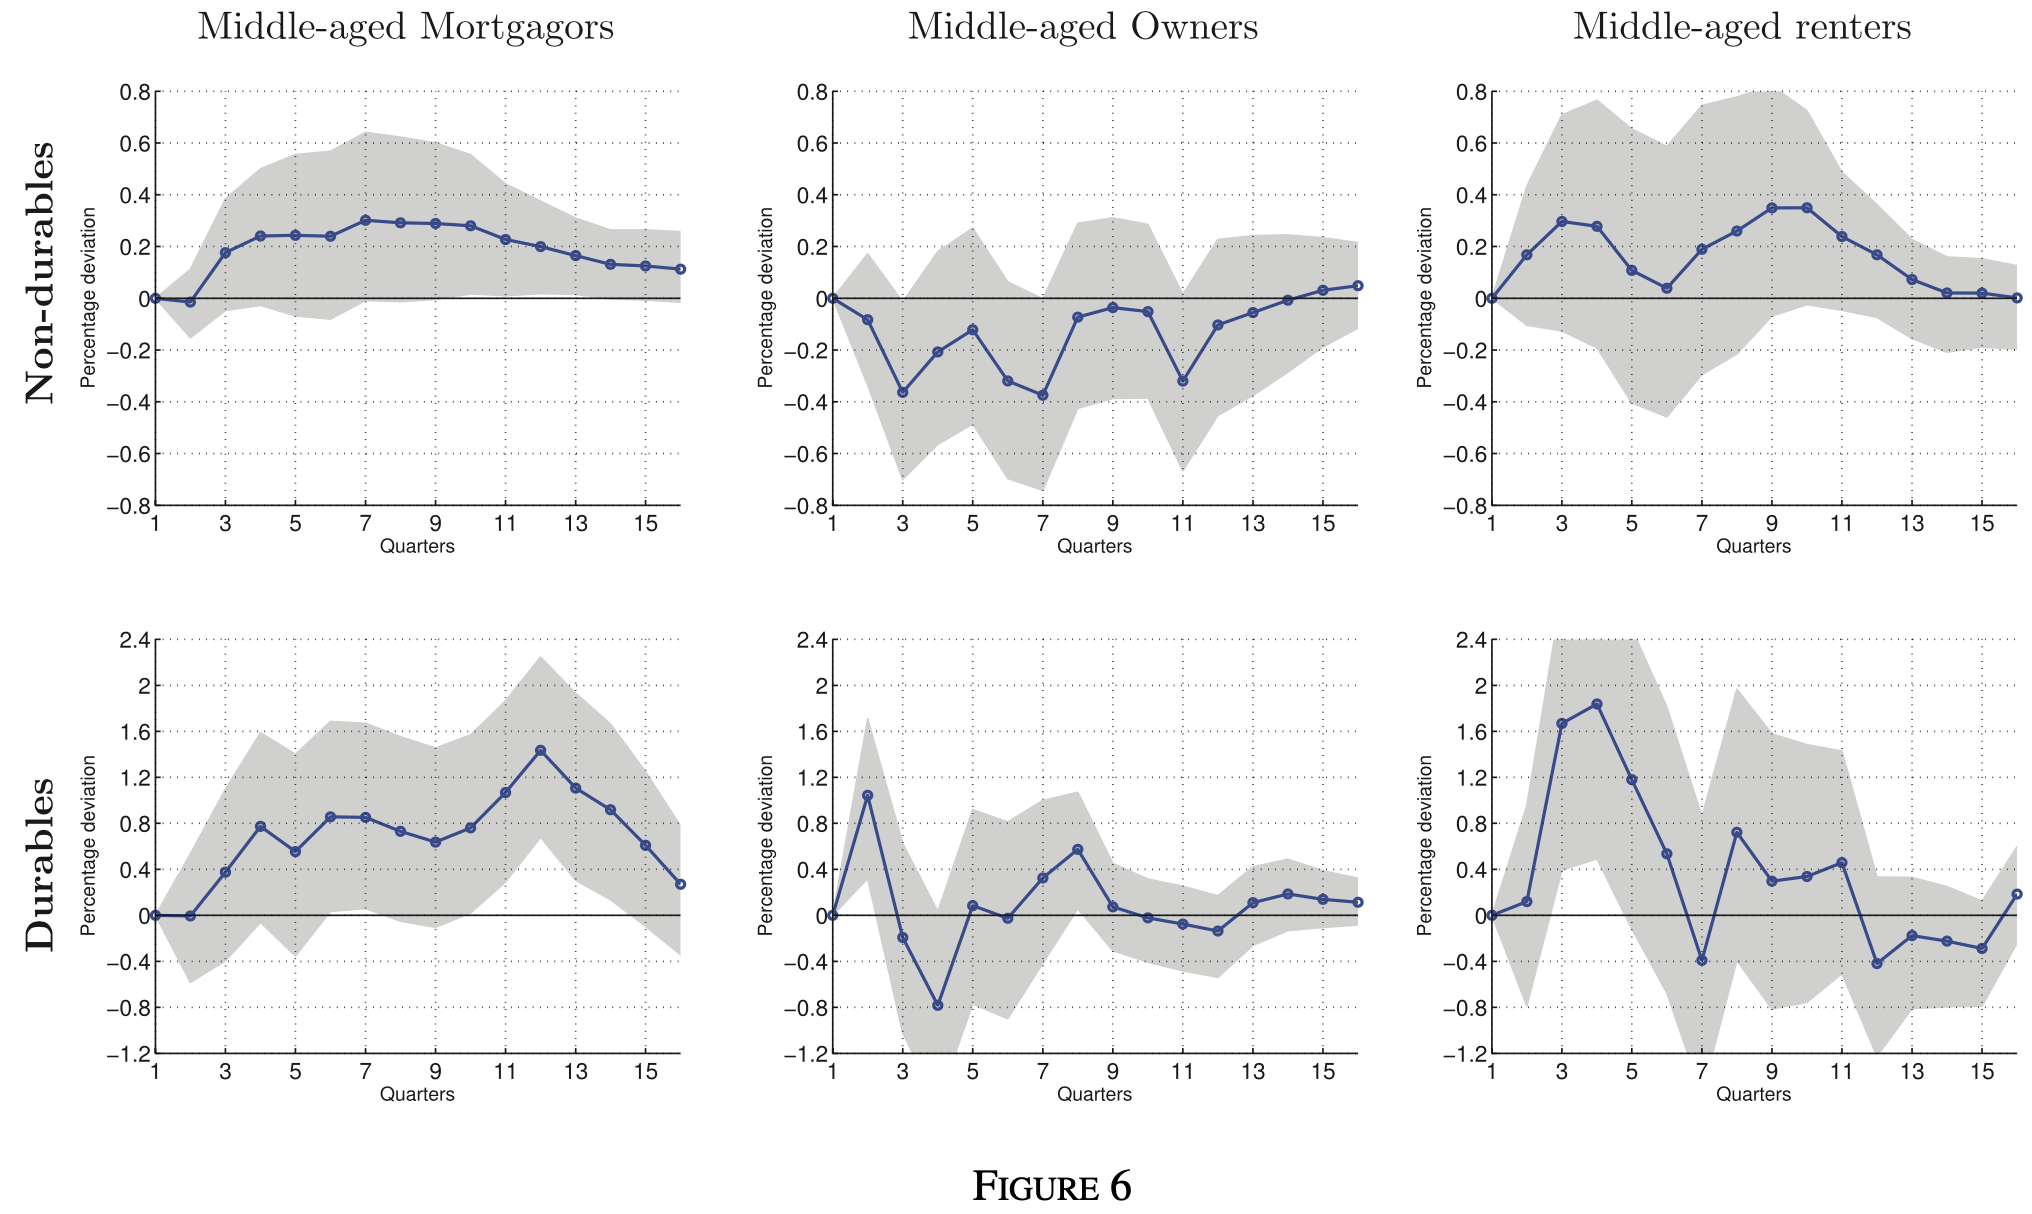
\includegraphics[scale=0.3]{figures/CFSFIG6.png}
% \end{frame}

% \begin{frame}
% \frametitle[alignment=center]{Convincing?}

% \end{frame}

% \begin{frame}
% \frametitle[alignment=center]{Questions}
% \begin{itemize}
% 	\item What is their preferred interpretation?
% 	\item What is causing the rise in income?
% \item What are the aggregate implications?
% 	\item How is it different from Hausman, Rhode, Wieland?
% \end{itemize}
% \end{frame}

%%%%%%%%%%%%%%%%%%%%%%%%%%%%%%%%%%%%%%%%%%%%%%%%%%
\section{Chodorow-Reich et al (2024, ReStud)}
%%%%%%%%%%%%%%%%%%%%%%%%%%%%%%%%%%%%%%%%%%%%%%%%%%

\begin{frame}
	\frametitle[alignment=center]{Housing}
	[graph of house prices]
	\begin{itemize}
		\item Bubble or Fundamentals? If fundamentals, demand or supply? (What is a fundamental?)
		\item Bubble view: Shiller, Charles et al
		\item Fundamental view: Chodorow-Reich et al, Mondragon and Wieland
		% \item Mian-Sufi: role of credit demand.
		% \item Credit supply: Primiceri paper
		% \item Chodorow-Reich et al: fundamentals.
		% \item Mondragon and Wieland: Covid demand.
	\end{itemize}
\end{frame}

\begin{frame}
	\frametitle[alignment=center]{Chodorow-Reich, Guren, McQuade (2024, ReStud)}
	\begin{enumerate}
		\item Document boom-bust-rebound.
		\item Fundamentals explain cross-city variation in long-run house price growth.
		\item Model that generates boom-bust-rebound from single fundamental shock with endogenous belief overreaction.
	\end{enumerate}
\end{frame}

\begin{frame}
	\frametitle[alignment=center]{Boom, Bust, and Rebound}
	\centering
	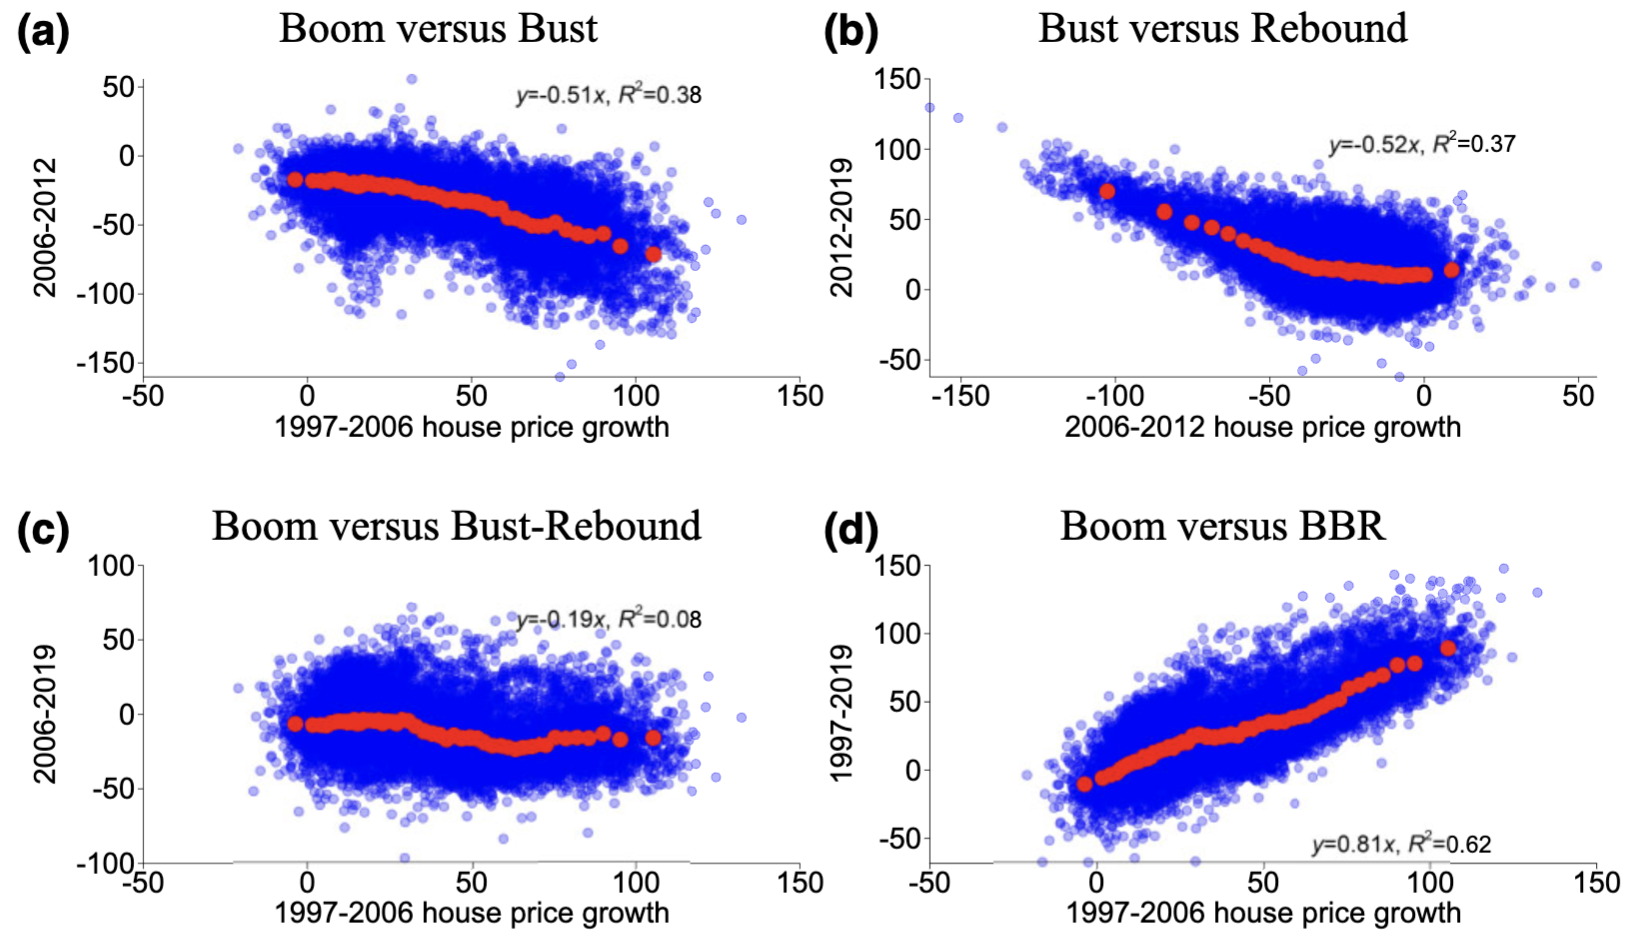
\includegraphics[scale=0.4]{figures/CGMFIG2.png}
\end{frame}

\begin{frame}
	\frametitle[alignment=center]{Framework for Long-Run Fundamentals}
	\begin{itemize}
		\item Good practice: write down the DGP.
		\item LR supply block:
		\begin{align*}
			P_{it} &= C_{it} + L_{it} \\
			C_{it} &= A_{it} H_{it}^{\alpha_i} \\
			L_{it} &= B_{it} H_{it}^{\beta_i} \\
		\end{align*}
		$A,B$ are cost shifters independent of population.
		\item LR demand block:
		\begin{align*}
			\frac{\dot{H}_{it}}{H_{it}} &= G_i \left(\frac{V_{it}}{P_{it}}\right)
			V_{it} &= E_t \int_t^\infty e^{-\rho s} D_{is}ds
		\end{align*}
	\end{itemize}
\end{frame}

\begin{frame}
	\frametitle[alignment=center]{Deriving LR Supply}
	\begin{itemize}
		\item Taking log differences with $s_{it}$ as the land share in $P$:
		\begin{align*}
			\Delta p_{it} &= \Delta a_{it} + s_{i,t-1} (\Delta b_{it} - \Delta a_{it}) + (\alpha_i + s_{i,t-1}(\beta_i - \alpha_i))h_{it}
		\end{align*}
		\item Parameterize:
		\begin{align*}
			\alpha_i &= \alpha_0 + \alpha_1 m_i \\
			\beta_i &= \beta_0 + \beta_1 m_i \\
			\Delta b_{it} &= b \Delta u_{it} + \Delta\bar{b}_t + \Delta\hat{b}_{it} \\
			\epsilon_{it} &= \Delta\hat{a}_{it} + s_{i,t-1} \Delta(\hat{b}_{it} - \Delta\hat{a}_{it})
		\end{align*}
		To get
		\begin{align*}
			\Delta p_{it} &= \Delta \bar{a}_{t} + s_{i,t-1}(\Delta\bar{b}_t-\Delta\bar{a}_t) +\alpha_0 \Delta h_{it} + (\beta_0 - \alpha_0 )s_{i,t-1}\Delta h_{it}  \\
			&+  \alpha_1 m_i \Delta h_{it} + (\beta_1 - \alpha_1)m_i s_{i,t-1}\Delta h_{it}+ s_{i,t-1}b\Delta u_{it} + \epsilon_{it}
		\end{align*}
		\item This becomes the regression equation
		\begin{align*}
			\Delta p_{it} = c_0 + s_{i,t-1}(\Delta\bar{b}_t-\Delta\bar{a}_t) +\alpha_0 \Delta h_{it} + (\beta_0 - \alpha_0 )s_{i,t-1}\Delta h_{it} \\
			&  +  \alpha_1 m_i \Delta h_{it} + (\beta_1 - \alpha_1)m_i s_{i,t-1}\Delta h_{it}+ s_{i,t-1}b\Delta u_{it} + \epsilon_{it}
		\end{align*}
	\end{itemize}
\end{frame}

\begin{frame}
	\frametitle[alignment=center]{Estimating LR Supply}
	\begin{itemize}
		\item This becomes the regression equation
		\begin{align*}
			\Delta p_{it} = c_0 + c_1 s_{i}  + c_2 \Delta h_{it} + c_3 s_{i}\Delta h_{it} \\
			&  +  c_4 m_i \Delta h_{it} + c_5 m_i s_{i,t-1}\Delta h_{it}+ c_6 s_{i} \Delta u_{it} + \epsilon_{it}
		\end{align*}
		(where are the $t$ subscripts on the coefficients?)
		\item Can we estimate this supply equation using OLS?
		
	\end{itemize}
\end{frame}

\begin{frame}
	\frametitle[alignment=center]{Instruments}
	\begin{itemize}
		\item Endogenous variables:
		\begin{itemize}
			\item Population growth $\Delta h_{it}$
			\item Land share $s_i$
			\item Regulatory strictness $m_i$
			\item Urbanization $\Delta u_{it}$
		\end{itemize}
		\item Instruments:
		\begin{itemize}
			\item Shift-share of employment growth and wage growth.
			\item January temperature and sunlight, July humidity.
			\item Share of employment in restaurants in 1997.
			\item Fraction of land available for development and 1997 population density.
			\item Ratio of public expenditure on protective inspection to total tax revenue in 1992, and share of Christians in non-traditional denominations in 1990.
			\item  The interaction of the pre-boom (1990) share of college workers
			in the CBSA and pre-boom urban amenities;  the interaction of the pre-boom relative likelihood of living downtown for college and non-college residents and the predicted change in the CBSA college share using a Bartik shift-share.
		\end{itemize}
		\item Thoughts? Comments?
	\end{itemize}
\end{frame}

\begin{frame}
	\frametitle[alignment=center]{Reduced Form}
	\centering
	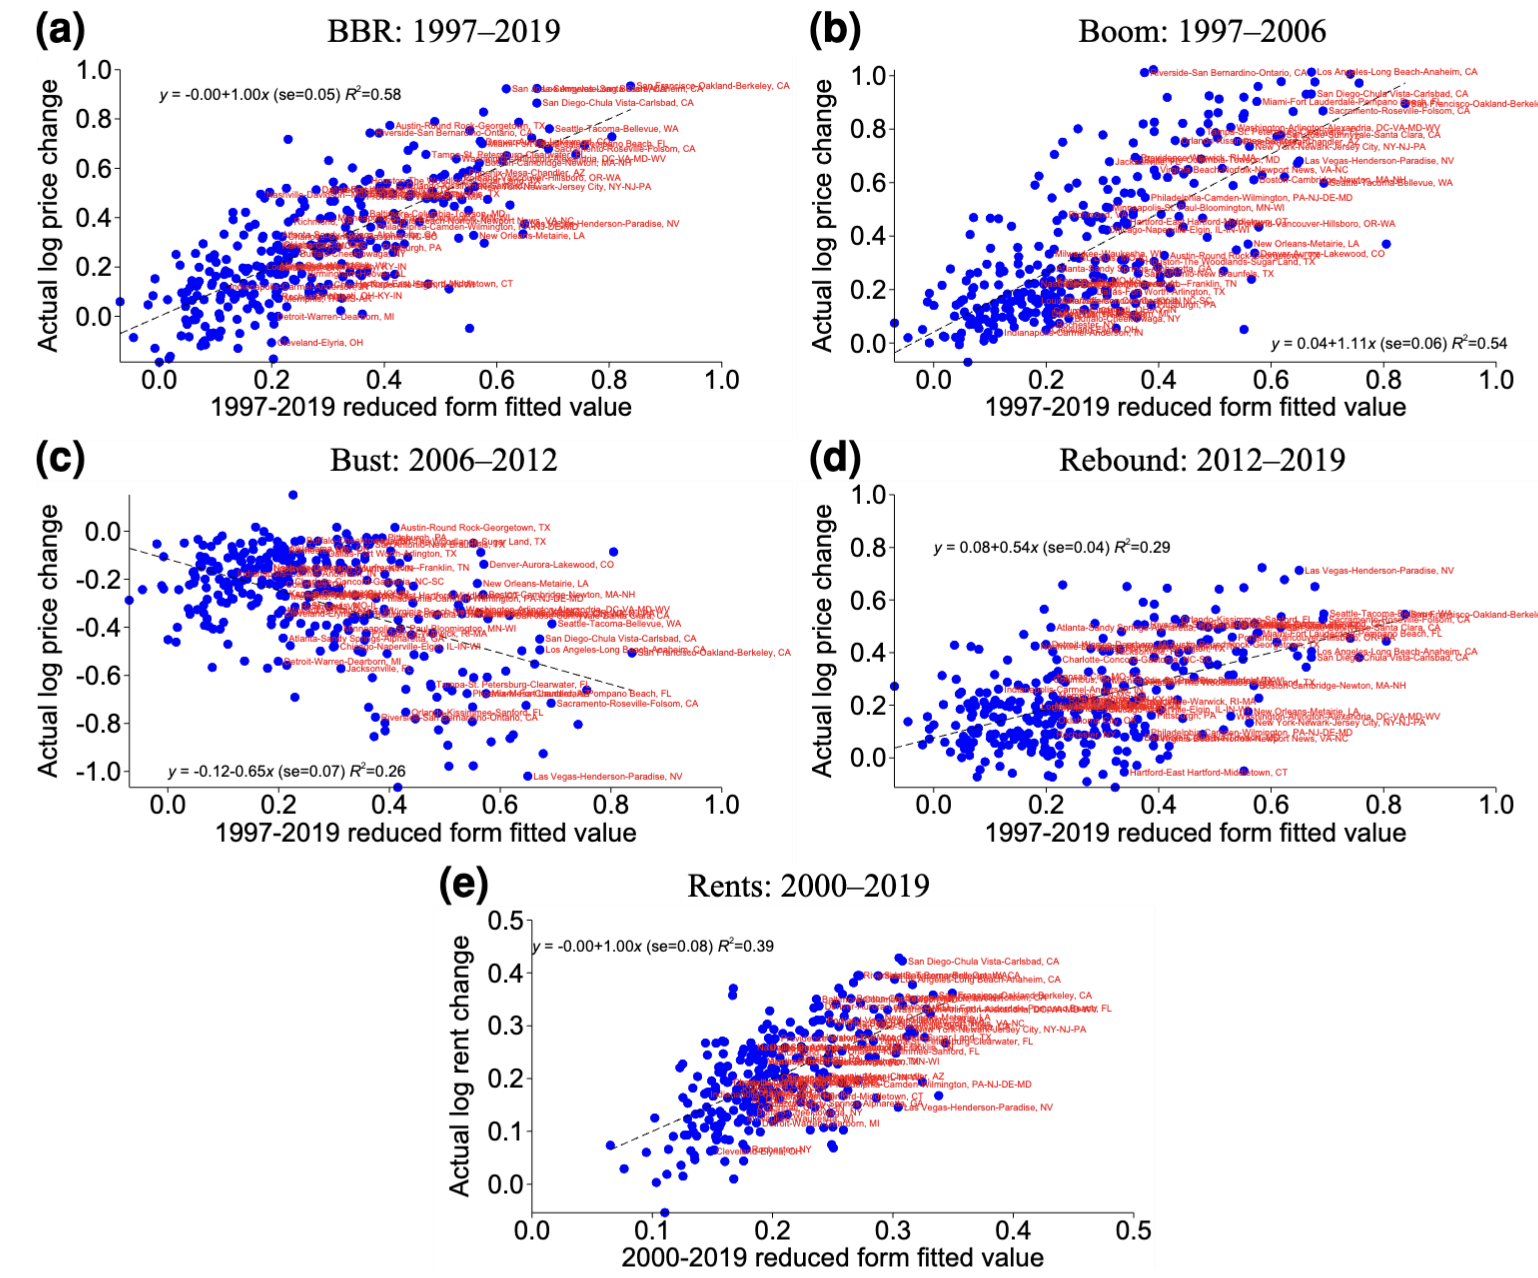
\includegraphics[scale=0.4]{figures/CGMFIG4.png}
\end{frame}

\begin{frame}
	\frametitle[alignment=center]{IV}
	\centering
	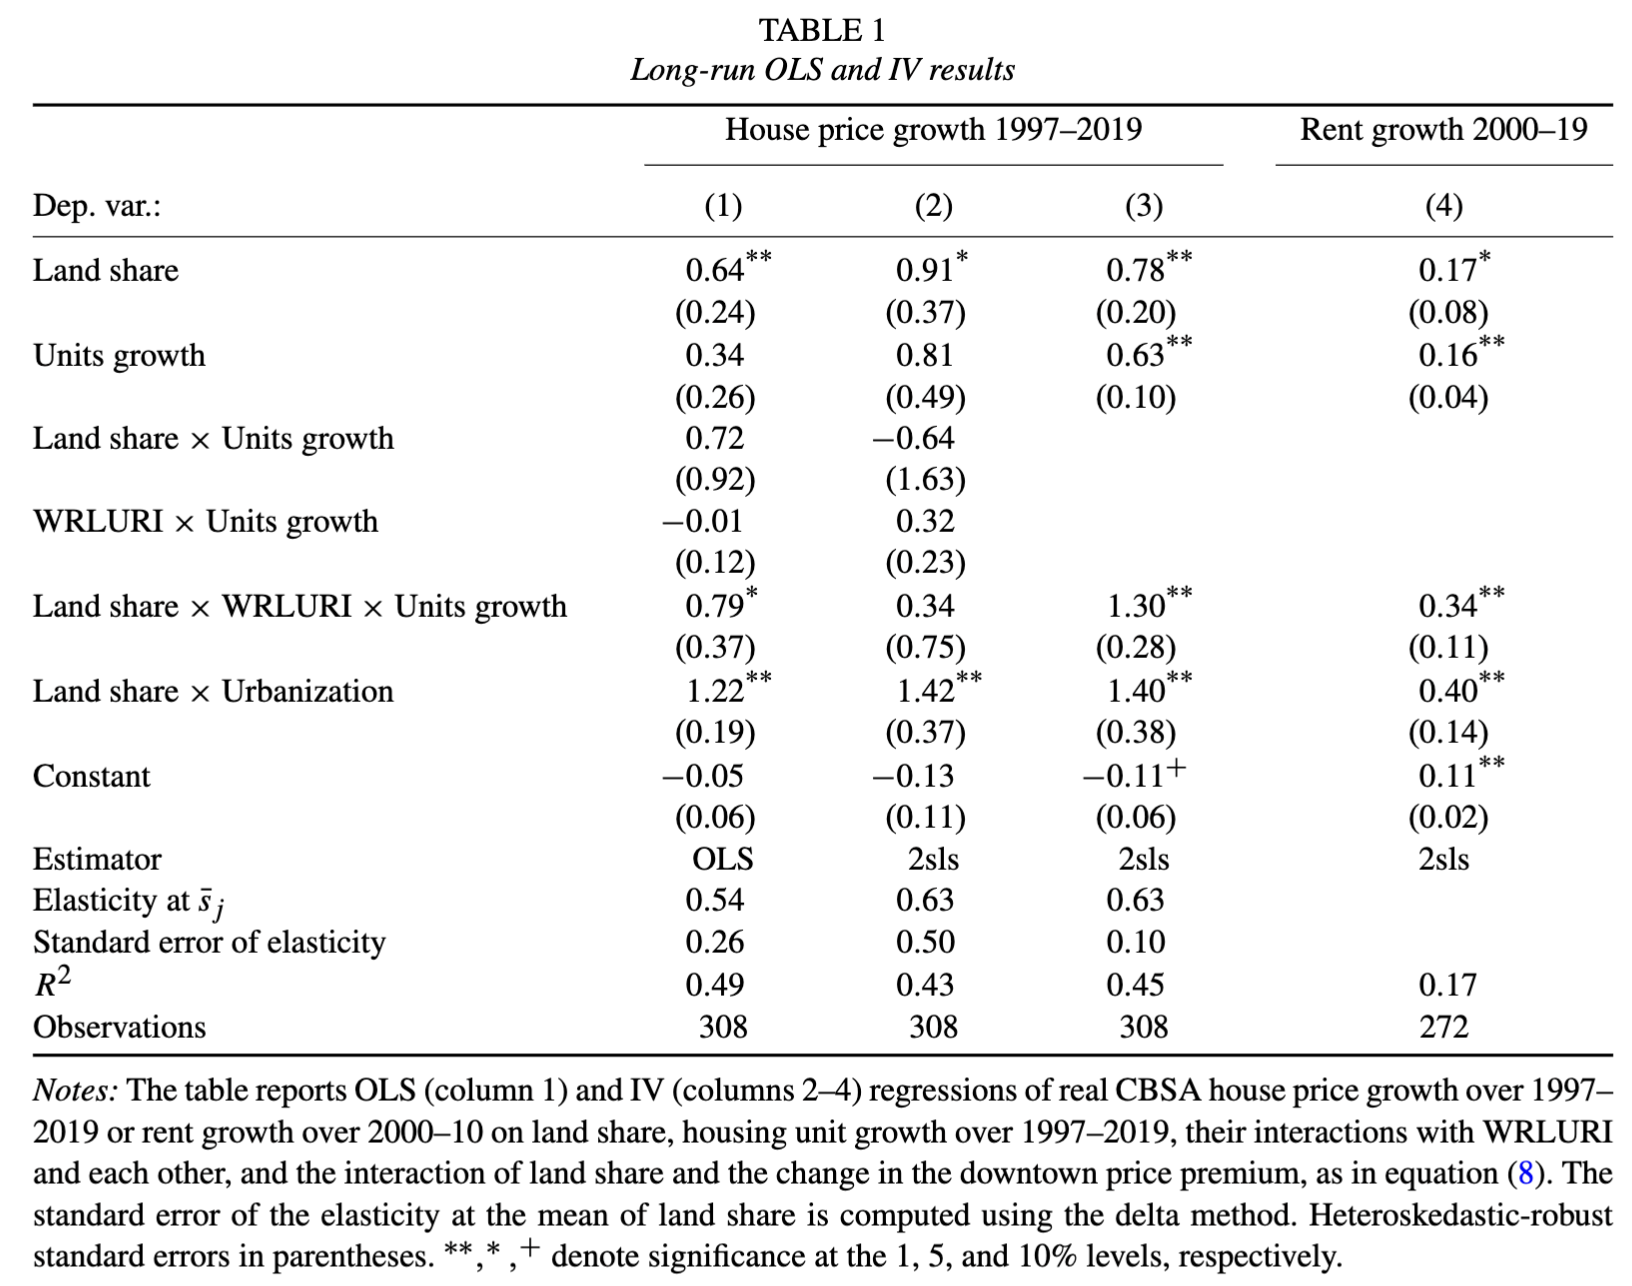
\includegraphics[scale=0.4]{figures/CGMTAB1.png}
	\begin{itemize}
		\item Comments? Concerns?
	\end{itemize}
\end{frame}

\begin{frame}
	\frametitle[alignment=center]{Loading on Fundamental}
	\centering
	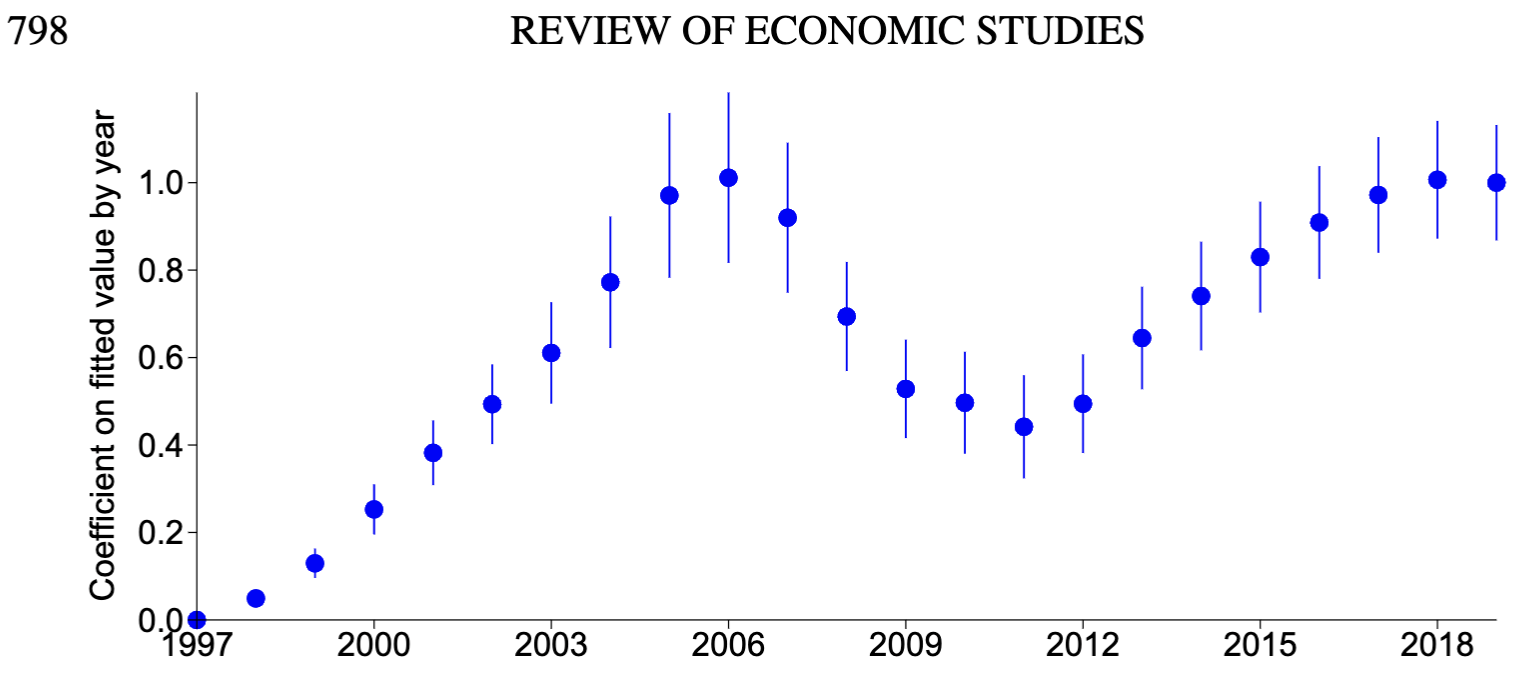
\includegraphics[scale=0.4]{figures/CGMFIG5.png}
	\begin{itemize}
		\item What do we learn?
	\end{itemize}
\end{frame}

\begin{frame}
	\frametitle[alignment=center]{Model}
	\begin{itemize}
		\item What is the purpose of the model?
		\item What do we learn from the model that we do not learn from the empirics?
		\item How well does the paper address the premise: fundamentals or bubbles?
	\end{itemize}
\end{frame}

\begin{frame}
	\frametitle[alignment=center]{Model}
	\centering
	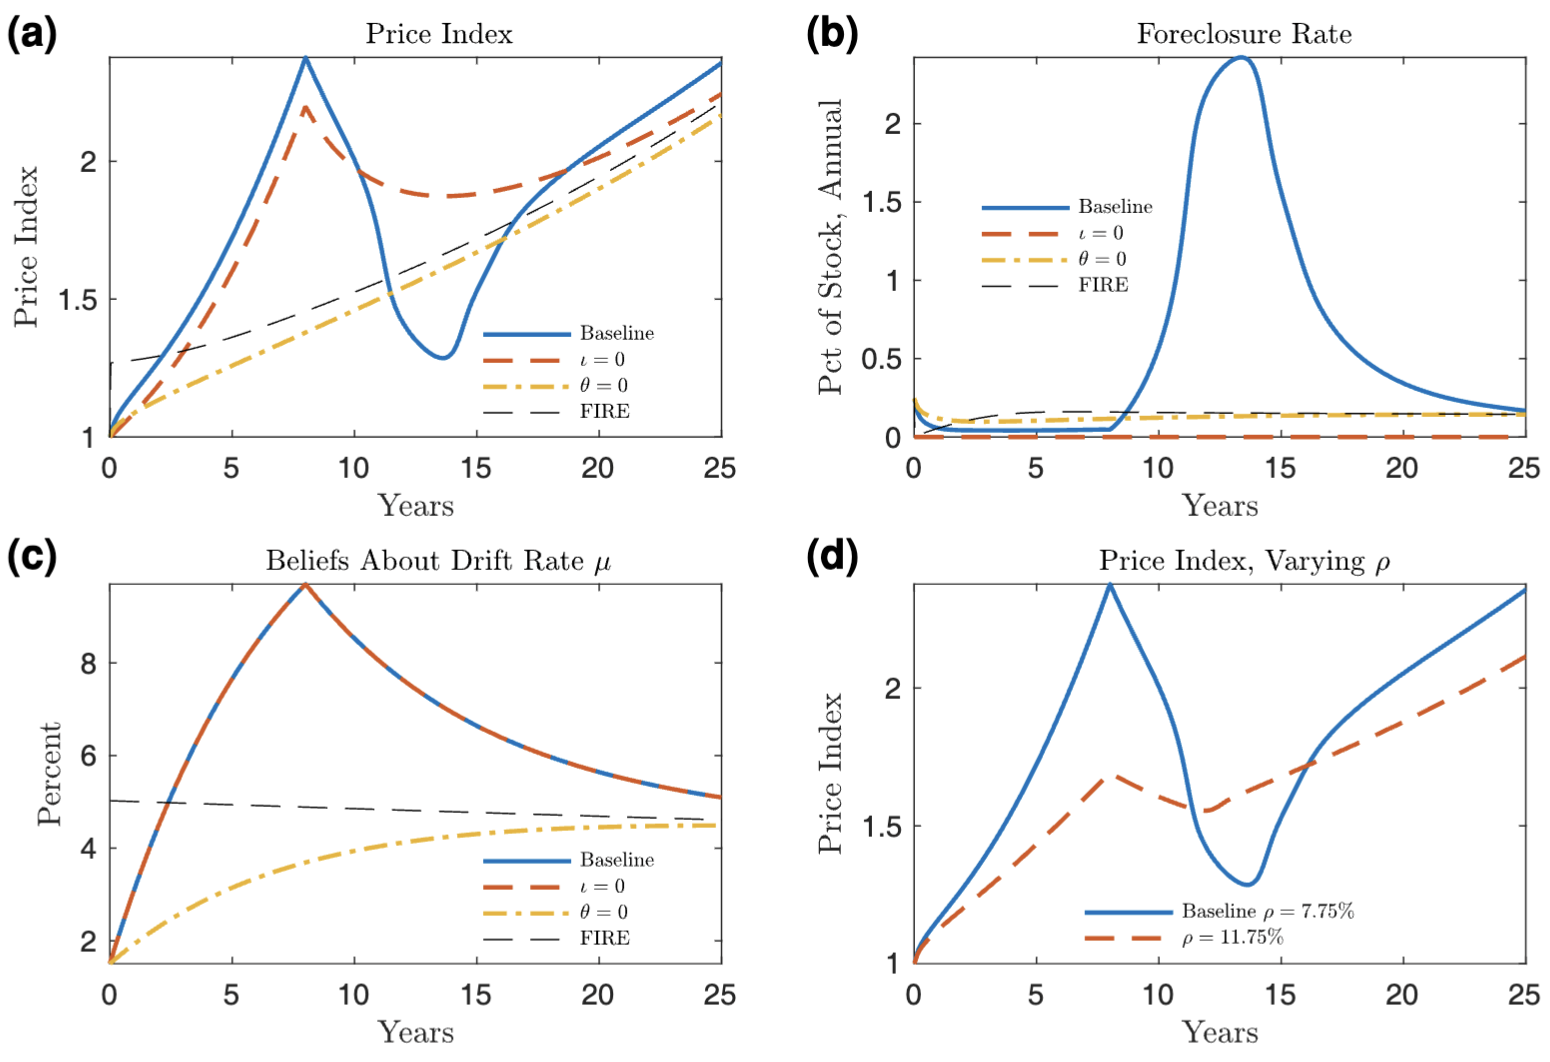
\includegraphics[scale=0.4]{figures/CGMFIG9.png}
\end{frame}

%%%%%%%%%%%%%%%%%%%%%%%%%%%%%%%%%%%%%%%%%%%%%%%%%%
\section{Mondragon and Wieland (2023, WP)}
%%%%%%%%%%%%%%%%%%%%%%%%%%%%%%%%%%%%%%%%%%%%%%%%%%

\end{document}